% Template for Elsevier CRC journal article
% Procedia Computer Science - ICMLDE 2026

\documentclass[3p,times,procedia]{elsarticle}
\flushbottom

%% The `ecrc' package must be called to make the CRC functionality available
\usepackage{ecrc}
\usepackage[bookmarks=false]{hyperref}
\hypersetup{colorlinks,
  linkcolor=blue,
  citecolor=blue,
  urlcolor=blue}
\usepackage{amssymb}
\usepackage{amsmath}
\usepackage{booktabs}
\usepackage{array}

%% ecrc package configurations
\volume{00}
\firstpage{1}
\journalname{Procedia Computer Science}
\runauth{[Author surname(s) to be confirmed]}
\jid{procs}

%% natbib options for numbered citations compliant with Procedia Vancouver style
\biboptions{sort&compress}

\begin{document}
\begin{frontmatter}

\dochead{5th International Conference on Machine Learning and Data Engineering}

\title{Source-Stratified Evaluation of Out-of-Distribution Detection in Fruit-Quality Classification Under Species and Treatment-Labelled Shifts}

\author[a]{Author Names Redacted for Peer Review}
\address[a]{[Department and Institution to be confirmed]}

\begin{abstract}
Automated fruit-quality classification using computer vision can achieve strong performance on familiar image distributions but may become unreliable under changes in data sources, fruit species, and post-harvest treatment conditions. This study presents a source-stratified empirical evaluation of a frozen MobileNetV2-based six-class fruit-quality classifier and multiple out-of-distribution (OOD) detection approaches. The evaluation uses 13,465 image records from three image repositories, organized into primary in-distribution, external known-class, unseen-species, treatment-labelled, and combined-shift cohorts.

Five established OOD scoring approaches---Maximum Softmax Probability (MSP), Energy, ODIN, Mahalanobis distance, and OpenMax---are compared with an operational Energy--MSP dual-gate cascade. Closed-set accuracy decreases from 96.92\% on the primary in-distribution test partition to 68.36\% on the pooled external known-class partition, reflecting a 28.56 percentage-point difference across evaluation sources. Within the FruitVision repository, Energy achieves an AUROC of 81.57\% for the known-versus-unseen-species comparison, with an operational false acceptance rate of 13.18\%, whereas the observed AUROC on the source-matched Sultana unseen-species comparison was 67.52\%. In the evaluated FruitVision treatment-labelled cohort, discrimination between natural known-class images and treatment-labelled known-class images is limited, with Energy achieving 53.13\% AUROC. Under fixed dual-gate operating thresholds calibrated on validation data, 42.83\% of the treatment-labelled image records are accepted and assigned a Fresh class.

The findings demonstrate that post-hoc OOD detection performance varies substantially across distribution shifts and data sources. In the evaluated treatment cohort, tested RGB post-hoc scoring methods did not reliably separate images recorded under the dataset-reported treatment protocol from natural fruit. The study provides an image-level benchmark analysis with source-stratified comparisons, uncertainty estimates, duplicate-sensitivity analysis, and explicit limitations concerning dataset labels, specimen independence, and operational validation.
\end{abstract}

\begin{keyword}
Fruit quality classification \sep Open-set recognition \sep Out-of-distribution detection \sep Domain shift \sep MobileNetV2 \sep Energy-based detection \sep Image classification \sep Food quality assessment
\end{keyword}

\cortext[cor1]{Corresponding author. E-mail: author@institution.edu}

\end{frontmatter}

\vspace*{-6pt}

%% Main document sections
\section{Introduction}
\label{sec:introduction}

\subsection{Research Background and Motivation}
\label{sec:background}
Post-harvest agricultural loss represents a critical challenge for global food security, economic stability, and supply chain sustainability \cite{fao2019state}. According to the Food and Agriculture Organization (FAO), approximately 14\% of global food production is lost between harvest and retail distribution \cite{fao2019state}. In regional agrarian economies, post-harvest deterioration across domestic transit corridors is particularly acute. For example, nationwide surveys in India conducted by the Indian Council of Agricultural Research (ICAR-CIPHET) indicate that post-harvest losses of commercial fruits consistently range between 6.70\% and 15.88\% (e.g., 10.39\% in apple, 7.76\% in banana, and 15.88\% in citrus) \cite{jha2015assessment}. These losses disproportionately penalize smallholder farmers and aggregation packhouses, where produce sorting and quality grading have historically relied upon manual, visual inspection. Manual grading is inherently subjective, labour-intensive, prone to operator fatigue, and incapable of scaling to high-throughput sorting facilities \cite{rizzo2023fruit,zhang2024fruit}.

In response to these operational bottlenecks, computer vision and deep learning have emerged as promising non-destructive methodologies for automated fruit freshness assessment, ripeness grading, and surface defect classification \cite{rizzo2023fruit,zhang2024fruit,chen2024classification,gulzar2023fruit}. Convolutional neural networks (CNNs), particularly lightweight architectures such as MobileNetV2 \cite{sandler2018mobilenetv2}, have become central to practical agricultural deployments. Depthwise separable convolutions and inverted residual bottlenecks allow MobileNetV2 to execute on resource-constrained mobile phones and edge sorting devices with parameter budgets under 4 million weights \cite{chen2024classification,sandler2018mobilenetv2}. In controlled academic benchmarks, modern visual classifiers routinely report top-1 accuracy exceeding 95\% across multi-class produce datasets \cite{zhang2024fruit,chen2024classification,gulzar2023fruit}.

\subsection{The Closed-Set Assumption and Its Vulnerabilities in Agricultural Vision}
\label{sec:closed_set_vulnerabilities}
Despite high benchmark accuracy, practical deployment of deep learning models in real-world agricultural environments encounters fundamental reliability barriers. Standard supervised image classifiers operate under a strict \textit{closed-set assumption}: the training, validation, and operational deployment data are presumed to be independent and identically distributed (i.i.d.) over a fixed, finite set of semantic classes, $\mathcal{Y} = \{1, 2, \dots, K\}$ \cite{guo2017calibration,hendrycks2017baseline}. In operational agricultural workflows, however, this assumption is persistently violated. Vision models deployed at packhouses, retail terminals, or farm collection centres confront three distinct, compounding categories of distribution shift:

\begin{enumerate}
\item \textbf{Covariate and Domain Shift:} Images collected across external facilities exhibit pronounced variations in background illumination, sensor optics, specular glare, ambient shadows, and post-harvest handling marks that differ markedly from laboratory training sets \cite{rizzo2023fruit,chen2024classification,abayomi2024fruitq,sultana2022extensive}. Furthermore, biological cultivar diversity---such as regional Asian apple varieties differing in pigmentation and surface russeting from Western commercial cultivars---induces domain shifts that degrade feature representations \cite{sultana2022extensive,bijoy2025fruitvision}.
\item \textbf{Semantic Shift (Unseen Species):} In automated sorting lines, bins, or field crates, models trained exclusively on a small palette of target crops (e.g., apple, banana, and orange) frequently encounter non-target produce species (e.g., mango, guava, jujube, pomegranate, or lime). Under standard closed-set inference, deep networks lack an explicit rejection mechanism; they are forced to assign an unseen species to one of the $K$ known classes, often with uncalibrated, erroneously high confidence \cite{guo2017calibration,hendrycks2017baseline}.
\item \textbf{Treatment-Labelled Condition Shift:} Horticultural commodities in post-harvest trade may undergo preservative treatments intended to retard visual senescence during extended storage or transit. In curated benchmarks such as FruitVision \cite{bijoy2025fruitvision}, images are documented under a specific post-harvest treatment protocol involving immersion in a 10\% formalin and 90\% water solution for 30 minutes, followed by drying and photography 48 hours later. When produce has undergone chemical treatment, superficial visual decay symptoms may be altered, altering the standard visual manifestations of biological freshness.
\end{enumerate}

Under standard softmax classification, neural networks are notoriously overconfident \cite{guo2017calibration}. Logit outputs normalized via the softmax function produce probability distributions that often peak sharply near 1.0 even when the input image is heavily corrupted, semantically anomalous, or completely out-of-distribution \cite{guo2017calibration,hendrycks2017baseline}. In agricultural supply chains, an overconfident false-positive classification---such as misclassifying an unseen non-target species or chemically treated decaying lot as ``Fresh Produce''---presents severe commercial, regulatory, and quality-assurance liabilities.

\subsection{Open-Set Recognition and Out-of-Distribution Detection Foundations}
\label{sec:osr_ood_foundations}
To address closed-set failure modes, computer vision research has developed two closely related paradigms: Open Set Recognition (OSR) \cite{scheirer2013toward,bendale2016towards} and Out-of-Distribution (OOD) Detection \cite{hendrycks2017baseline,yang2024generalized}. 

The concept of open-set recognition was formalized by Scheirer et al. \cite{scheirer2013toward}, who defined the objective as simultaneously classifying known training classes while bounding the open space risk---the risk of incorrectly labeling an unknown, novel class sample as any known class. Bendale and Boult \cite{bendale2016towards} extended this concept to deep neural networks through OpenMax, which estimates the probability of an input belonging to an unknown class by fitting Weibull distributions to activation vectors in the penultimate layer.

Simultaneously, the broader machine learning community formalized generalized out-of-distribution detection \cite{hendrycks2017baseline,yang2024generalized}. Hendrycks and Gimpel \cite{hendrycks2017baseline} established the Maximum Softmax Probability (MSP) baseline, showing that correctly classified in-distribution samples typically exhibit higher maximum posterior probabilities than anomalous inputs. Liang et al. \cite{liang2018enhancing} developed ODIN, which amplifies the separation between in-distribution and out-of-distribution samples using temperature-scaled softmax outputs and input-space gradient perturbations. Lee et al. \cite{lee2018simple} introduced a feature-space Mahalanobis distance metric that models class-conditional Gaussian distributions across intermediate hidden representations. More recently, Liu et al. \cite{liu2020energy} proposed Energy-based OOD detection, utilizing the Helmholtz free energy function computed directly over unnormalized logits. Energy scores possess the theoretical advantage of being linearly aligned with the true input marginal probability density, avoiding the artificial probability saturation inherent in softmax normalization \cite{yang2024generalized,liu2020energy}. Additionally, Vaze et al. \cite{vaze2022open} demonstrated that closed-set classifier capacity and representation quality strongly dictate open-set discrimination performance.

In operational deployment, OOD detectors are typically implemented either as continuous ranking functions or as discrete rejection gates governed by a pre-calibrated threshold $\tau$. When an input sample produces an anomaly score that violates the threshold, the system abstains from classification, triggering manual inspection or secondary non-optical assay.

\subsection{Prior Agricultural OSR/OOD Studies and Specific Research Gaps}
\label{sec:prior_work_gaps}
Open-set recognition and anomaly detection have recently attracted growing attention in agricultural vision. Several recent investigations have examined related challenges:
\begin{itemize}
\item Sattar et al. \cite{sattar2024sensornet} developed SensorNet, combining computer vision, deep learning, and chemical sensors to identify chemical adulteration in fruit specimens.
\item Bijoy et al. \cite{bijoy2025fruitvision} introduced FruitVision, an image dataset containing fresh, rotten, and formalin-mixed fruit images.
\item Wang et al. \cite{wang2023crossdomain} proposed lightweight attention networks with unsupervised domain adaptation for cross-domain fruit classification.
\item Pehlivan and Kara \cite{pehlivan2026lightweight} introduced a lightweight one-shot open-set metric learning framework for food recognition in smart appliances.
\item Jansi and Kavitha \cite{jansi2026peos} developed PEOS-Net, an evidential open-set framework for plant leaf disease recognition.
\item Yan et al. \cite{yan2026pagmsbnet} formulated PAG-MSBNet, using prototype-augmented graphs for open-set crop disease recognition.
\end{itemize}

While these studies highlight the importance of non-standard conditions in agricultural classification, existing research has not systematically evaluated how established post-hoc OOD scoring functions behave when a frozen classifier faces multi-source external distributions. Specifically, four key empirical gaps remain:

\begin{enumerate}
\item \textbf{Gap 1: Over-Optimistic Internal-Split Benchmarks:} The majority of existing fruit-freshness studies report classification and anomaly detection metrics computed exclusively on random train/test splits of a single, curated dataset \cite{zhang2024fruit,chen2024classification,gulzar2023fruit}. Audits reveal that random image partitioning in agricultural benchmarks frequently suffers from near-duplicate and affine leakage between training and testing sets, producing inflated accuracies that fail to generalize to external repositories \cite{abayomi2024fruitq,sultana2022extensive}.
\item \textbf{Gap 2: Cross-Repository Confounding in OOD Benchmarks:} When external evaluations are conducted, researchers commonly evaluate unseen species drawn from a completely different repository than the known-class training cohort. This experimental design introduces severe \textit{cross-repository confounding}: the detector's ability to reject the unseen species is driven largely by differences in camera hardware, studio lighting, and background compression rather than true biological or semantic divergence \cite{yang2024generalized}. Without \textit{source-stratified} benchmarks that evaluate known and unknown produce collected under identical repository conditions, the true semantic discrimination capacity of vision models remains unmeasured.
\item \textbf{Gap 3: Empirical Behavior Under Treatment-Labelled Shifts:} While multi-modal sensing has explored chemical adulteration \cite{sattar2024sensornet}, no prior study has systematically evaluated whether post-hoc OOD detection methods applied to standard RGB classifiers can discriminate between naturally fresh fruit and produce documented under chemical immersion protocols \cite{bijoy2025fruitvision}.
\item \textbf{Gap 4: Retrospective Metric Optimism vs. Operational Threshold Reliability:} Nearly all published OOD literature evaluates algorithms using threshold-free retrospective metrics, specifically the Area Under the Receiver Operating Characteristic curve (AUROC) and the False Positive Rate at 95\% True Positive Rate (FPR@95) \cite{hendrycks2017baseline,yang2024generalized,liu2020energy}. While informative for theoretical comparison, retrospective metrics assume oracle access to the entire test distribution. In real-world sorting, systems must operate prospectively with \textit{fixed thresholds} pre-calibrated on internal validation sets. The degree to which fixed validation thresholds maintain acceptable Unknown False Acceptance Rates (UFAR) without causing severe Known-Class Rejection Rates (KRR) on external produce has not been rigorously quantified.
\end{enumerate}

\subsection{Research Objectives and Formal Research Questions}
\label{sec:research_questions}
This investigation addresses these gaps by conducting an extensive, source-stratified empirical evaluation of out-of-distribution detection in fruit image classification. The study evaluates a frozen MobileNetV2 six-class visual classifier across $N = 13,465$ image records curated from three distinct repositories under the Stage 4.0.3 external evaluation protocol. 

The paper specifically investigates three core research questions:
\begin{itemize}
\item \textbf{Research Question 1 (RQ1 --- External Generalization):} How does the closed-set classification performance (top-1 accuracy, macro-F1, and balanced accuracy) of a lightweight MobileNetV2 model change when evaluated on external repositories containing the same known fruit classes?
\item \textbf{Research Question 2 (RQ2 --- OOD Discrimination):} How effectively do established OOD scoring mechanisms (MSP, Energy, ODIN, Mahalanobis distance, OpenMax) discriminate between in-distribution produce and distribution shifts when evaluated in source-matched cohorts isolating (a) unseen-species semantic shift, (b) treatment-labelled condition shift, and (c) combined species-and-treatment shifts?
\item \textbf{Research Question 3 (RQ3 --- Operational Reliability):} How do fixed validation-calibrated rejection thresholds ($\tau_{95}$) affect out-of-distribution false acceptance (UFAR) and known-class retention (KRR) under external domain and condition shifts?
\end{itemize}

\subsection{Evidence-Supported Research Contributions}
\label{sec:contributions}
The primary contribution of this work is an empirical source-stratified evaluation, rigorous uncertainty audit, and diagnostic failure analysis. The study does not propose a novel standalone OOD algorithm, nor does it claim real-world agricultural supply chain deployment. The four specific, evidence-backed contributions of this study are:

\begin{enumerate}
\item \textbf{Audited Source-Stratified Benchmark Census ($N = 13,465$):} We establish an audited image-level evaluation benchmark comprising 13,465 image records structured across five distinct partitions: Partition A (Primary ID Test, $N=227$), Partition B (External Known-Class Shift, $N=5,350$), Partition C (Treatment-Labelled Condition Shift, $N=1,917$), Partition D1 (Unseen-Species Shift, $N=4,776$), and Partition D2 (Combined Shift, $N=1,195$). We incorporate exact-duplicate handling and perceptual-hash (pHash) sensitivity analysis across Hamming distance radii $r \in \{0, 4, 8\}$.
\item \textbf{Quantification of Closed-Set Domain Collapse:} We demonstrate that the frozen MobileNetV2 backbone undergoes a 28.56 percentage-point drop in top-1 accuracy---collapsing from 96.92\% [94.71\%, 98.68\%] on the laboratory test partition (Partition A) to 68.36\% [67.20\%, 69.40\%] on pooled external retail fruit (Partition B), with balanced accuracy decreasing from 97.09\% to 68.66\%. Through source stratification, we show that performance varies across external repositories (FruitVision B: 69.14\% accuracy, 69.56\% balanced accuracy; Sultana B: 65.63\% accuracy, 65.55\% balanced accuracy), with misclassifications heavily concentrated in russeted fresh apples and pale citrus cultivars.
\item \textbf{Source-Matched Isolation of Semantic vs. Treatment Shifts:} By benchmarking within shared repositories, source matching reduces cross-repository confounding while potential within-repository capture variation remains. We show that while Energy-based detection achieves robust discrimination under Within-FruitVision semantic shift (Cohort A: 81.57\% AUROC [80.81\%, 82.38\%], 13.18\% operational UFAR), discrimination degrades significantly on external cultivars with visual overlap (Within-Sultana Cohort D: 67.52\% AUROC [65.67\%, 69.25\%], 34.90\% operational UFAR).
\item \textbf{Empirical Diagnosis of Treatment Shift Failure and Operational Trade-Offs:} We demonstrate that standard RGB post-hoc OOD detectors fail to reliably distinguish produce documented under chemical immersion protocols from natural known fruit (Within-FruitVision Cohort B: Energy AUROC of only 53.13\% [52.16\%, 54.09\%]). Under locked validation operating thresholds ($\tau_{95}$), the Dual-Gate cascade yields an operational UFAR-Fresh of 42.83\% [41.26\%, 44.34\%] ($821/1,917$ images) on the treatment-labelled cohort, demonstrating that RGB image features alone cannot reliably identify this condition. Furthermore, we reveal that maintaining an operational UFAR of 16.07\% on external produce incurs an in-distribution known-class false rejection rate (KRR) of approximately 41.98\% ($2,246/5,350$ images).
\end{enumerate}


\section{Related Work}
\label{sec:related_work}

This section will provide a detailed review of literature covering: (1) deep learning applications in post-harvest fruit quality assessment and freshness classification; (2) open-set recognition and generalized out-of-distribution detection algorithms; and (3) distribution shifts and domain adaptation techniques in agricultural vision systems.


\section{Dataset Census and Experimental Design}
\label{sec:dataset_design}

This section details the source-stratified evaluation benchmark, comprising $N = 13,465$ audited photographic image records assembled from three independent repositories. We present the study design rationale, repository provenance, label-mapping protocol, five-partition census, four source-matched evaluation cohorts, duplicate and perceptual-hash sensitivity analysis, experimental separation safeguards, and reproducibility artifacts.

\subsection{Study Design Overview}
\label{sec:study_design_overview}

Evaluating automated fruit-quality classification models under practical deployment conditions presents a complex experimental challenge. When vision models trained on curated image datasets are evaluated on external imagery, observed performance degradation typically reflects multiple confounding factors acting simultaneously: variations in camera sensor optics, ambient illumination, photographic backgrounds, biological cultivars, and post-harvest handling marks \cite{abayomi2024fruitq,sultana2022extensive,bijoy2025fruitvision}. If images from diverse sources are simply pooled into an aggregated test set, it becomes impossible to determine whether detection failures stem from semantic novelty (encountering an unseen fruit species), physiological or surface anomalies (encountering damaged or chemically treated produce), or mere covariate shift in image acquisition conditions.

To resolve these compounding factors, this study implements a \textit{source-stratified empirical evaluation}. We freeze a pre-trained six-class MobileNetV2 classifier \cite{sandler2018mobilenetv2} and evaluate it across structured image cohorts drawn from three independent repositories: the Primary Kaggle dataset, FruitVision \cite{bijoy2025fruitvision}, and Sultana et al. \cite{sultana2022extensive}. Crucially, the experimental architecture maintains a strict distinction between:
\begin{enumerate}
\item \textbf{Closed-Set Generalization (Partitions A and B):} Evaluating accuracy, balanced accuracy, and class-wise confusion on known classes across laboratory baseline conditions (Partition A, $N = 227$) versus external retail and field environments (Partition B, $N = 5,350$), holding the label space $\mathcal{Y} = \{0, 1, \dots, 5\}$ constant.
\item \textbf{Out-of-Distribution Detection (Partitions C, D1, and D2):} Evaluating the capacity of post-hoc scoring functions to detect and reject non-target inputs, including treatment-labelled condition shifts (Partition C, $N = 1,917$), unseen fruit species (Partition D1, $N = 4,776$), and compound shifts (Partition D2, $N = 1,195$).
\end{enumerate}

Furthermore, to separate the specific mechanism of out-of-distribution (OOD) shift from cross-repository acquisition bias, we structure the OOD evaluation into four \textit{source-matched cohorts} (Cohorts A, B, C, and D). By comparing in-distribution known images and out-of-distribution anomalous images collected within the same parent repository, source matching reduces repository-level provenance differences, while within-repository acquisition variation remains possible. Throughout this study, the evaluation unit is designated strictly as an \textit{image record}; photographic records cannot be assumed to represent statistically independent biological specimens.

\subsection{Dataset Sources and Provenance}
\label{sec:dataset_sources_provenance}

The benchmark image census is compiled from three independent photographic archives, each characterized by distinct acquisition settings, camera modalities, and environmental conditions. Table~\ref{tab:dataset_provenance} summarizes the provenance, published composition, evaluated subsets, and key characteristics of each repository.

\begin{table*}[!t]
\caption{Dataset source and provenance summary. Evaluated record counts represent audited, unique image records included in the present study after hash-identified duplicate removal, distinguishing local benchmark subsets from published repository totals.}
\label{tab:dataset_provenance}
\centering
\footnotesize
\setlength{\tabcolsep}{2.5pt}
\begin{tabular}{>{\raggedright\arraybackslash}p{2.3cm} >{\raggedright\arraybackslash}p{2.2cm} >{\raggedright\arraybackslash}p{2.3cm} >{\centering\arraybackslash}p{1.3cm} >{\raggedright\arraybackslash}p{2.5cm} >{\raggedright\arraybackslash}p{4.2cm}}
\toprule
\textbf{Source Repository} & \textbf{Citation / Venue} & \textbf{Published Composition} & \textbf{Evaluated $N$} & \textbf{Evaluated Species \& Conditions} & \textbf{Capture Environment \& Key Provenance} \\
\midrule
Primary Kaggle Archive & Curated public benchmark & 2,043 test images \newline (227 raw, 1,816 aug.) & 227 & Apple, banana, orange \newline (Fresh, Rotten) & Controlled laboratory-style conditions with uniform backgrounds; neutral illumination; baseline ID test set (Partition A). \\
\addlinespace[3pt]
FruitVision & Bijoy et al. (2025) \cite{bijoy2025fruitvision} \newline \textit{Data in Brief} & 10,154 raw images \newline (81,232 aug. archive) & 10,045 & Apple, banana, orange, grape, mango \newline (Fresh, Rotten, Formalin-mixed) & 3 mobile smartphone cameras (Samsung A50, Redmi Note 7, iPhone 11); indoor/outdoor retail lighting; 109 hash-identified duplicates excluded. \\
\addlinespace[3pt]
Sultana et al. & Sultana et al. (2022) \cite{sultana2022extensive} \newline \textit{Data in Brief} & 16 classes, 8 fruits \newline ($\sim$3,200 raw images) & 3,193 & Apple, banana, orange, grape, guava, jujube, pomegranate, strawberry \newline (Fresh, Rotten) & Retail fruit shops and open agricultural fields; natural ambient illumination; agricultural specialist annotation; 7 hash-identified duplicates excluded. \\
\midrule
\textbf{Total Benchmark} & \textbf{Three Repositories} & \textbf{Multiple Archives} & \textbf{13,465} & \textbf{8 Fruit Species, 3 Conditions} & \textbf{Audited multi-source evaluation census (Partitions A--D2).} \\
\bottomrule
\end{tabular}
\end{table*}

\subsubsection{Primary Kaggle Dataset}
The primary training and baseline evaluation partition originates from a widely utilized curated benchmark repository for fruit freshness classification. The repository covers three commercial fruit types---apple (\textit{Malus domestica}), banana (\textit{Musa acuminata}), and orange (\textit{Citrus sinensis})---each categorized into fresh and rotten states. Photography was conducted under controlled laboratory-style conditions with relatively uniform, neutral backgrounds and stable illumination. The published test partition contains 2,043 files consisting of 227 raw photographic images and 1,816 synthetic geometric and photometric augmentations. In this study, we strictly isolate the 227 raw, unaugmented photographic images (`\texttt{is\_raw == 1}') to construct Partition A (Primary In-Distribution Test). The 1,816 synthetically augmented images were set aside to restrict evaluation strictly to authentic photographic captures; these represent upstream synthetic transformations and are not classified as duplicate removals. An independent validation partition of 227 raw images was maintained strictly for operating-threshold calibration (see Section~\ref{sec:evaluation_integrity}).

\subsubsection{FruitVision Repository}
The FruitVision dataset was introduced by Bijoy et al. \cite{bijoy2025fruitvision} as a benchmark for produce freshness, rot, and adulteration recognition. The repository encompasses five fruit species: three known species (apple, banana, orange) and two non-target species (grape \textit{Vitis vinifera} and mango \textit{Mangifera indica}). Photography was conducted across diverse wholesale markets, retail stalls, and laboratory benches using three commercial smartphone devices: Samsung Galaxy A50 (25\,MP primary sensor), Xiaomi Redmi Note 7 (48\,MP primary sensor), and Apple iPhone 11 (12\,MP primary sensor). Image capture spanned varied ambient indoor lighting, direct outdoor sunlight, and fluorescent retail illumination. 

A distinctive feature of FruitVision is its inclusion of a dataset-reported treatment protocol: fruits were immersed in a solution of 10\% formalin and 90\% water for 30 minutes, allowed to air-dry, and photographed 48 hours post-immersion under natural ambient conditions alongside untreated fresh and naturally decaying specimens. While Bijoy et al. published 10,154 raw photographs (expanded via photometric and geometric transformations to an 81,232-image augmented archive), the present study extracts exclusively the raw photographic collection. Cryptographic hash auditing identified and removed 109 hash-identified duplicate files, yielding exactly 10,045 audited image records evaluated across Partitions B, C, D1, and D2. We emphasize that treatment-labelled images are evaluated strictly under their dataset-reported labels; no independent chemical assays or residue validations were conducted.

\subsubsection{Sultana et al. Repository}
The dataset introduced by Sultana et al. \cite{sultana2022extensive} was curated to recognize produce quality across authentic retail and farm environments. The dataset contains 16 fresh and rotten categories representing eight distinct fruit species: apple, banana, orange, grape, guava (\textit{Psidium guajava}), jujube (\textit{Ziziphus jujuba}), pomegranate (\textit{Punica granatum}), and strawberry (\textit{Fragaria $\times$ ananassa}). Images were captured in local retail shops and active agricultural orchards under ambient natural lighting, with fruit specimen selection and freshness categorization verified with assistance from an agricultural domain specialist. We harvested 3,200 raw photographic records (200 records per class across all 16 classes). MD5 cryptographic hashing identified 7 hash-identified duplicate files within the orange fresh class, leaving exactly 3,193 audited image records evaluated across Partitions B and D1.

\subsection{Known-Class Definition and Label Mapping}
\label{sec:known_class_mapping}

The classification space of the frozen MobileNetV2 backbone is defined over $K = 6$ discrete semantic classes:
\begin{equation}
\begin{aligned}
\mathcal{Y} = \{ & 0: \text{fresh\_apple}, \; 1: \text{fresh\_banana}, \; 2: \text{fresh\_orange}, \\
                 & 3: \text{rotten\_apple}, \; 4: \text{rotten\_banana}, \; 5: \text{rotten\_orange} \}.
\end{aligned}
\end{equation}

To integrate external imagery into this framework, we apply unambiguous label-mapping rules governed by the underlying biological species and physical freshness condition:
\begin{enumerate}
\item \textbf{External Known-Class Mapping (Partition B):} External images from FruitVision and Sultana et al. depicting apple, banana, or orange in natural fresh or rotten states are mapped directly to their corresponding index in $\mathcal{Y}$. For example, FruitVision \texttt{Fresh\_Apple} maps to class 0, and Sultana \texttt{rotten\_orange} maps to class 5. No class collapsing across fresh/rotten boundaries or cross-species reassignments are permitted.
\item \textbf{Unseen-Species OOD Mapping (Partition D1):} Images depicting botanical species outside the set $\{\text{apple}, \text{banana}, \text{orange}\}$ in natural fresh or rotten conditions are designated as out-of-distribution unseen species. This includes grape and mango from FruitVision, and grape, guava, jujube, pomegranate, and strawberry from Sultana et al.
\item \textbf{Treatment-Labelled Condition Shift Mapping (Partition C):} Images from FruitVision depicting known species (apple, banana, orange) photographed under the dataset-reported formalin-immersion condition are designated as treatment-labelled condition shifts. Because the classifier was trained exclusively on untreated produce, these images evaluate whether post-hoc OOD scoring functions discriminate images bearing the dataset-reported treatment label from untreated knowns. This evaluation tests model behavior on produce labelled under altered post-harvest handling; it does not claim independent chemical detection, residue verification, or the establishment of treatment-caused visual anomalies.
\item \textbf{Combined Shift Mapping (Partition D2):} Images from FruitVision depicting unseen species (grape and mango) subjected to the dataset-reported formalin-immersion condition are designated as combined shifts, presenting simultaneous semantic and treatment condition divergence.
\end{enumerate}

No subjective manual pruning or post-hoc relabeling was performed; all annotations adhere strictly to the verified manifests of the respective source publications.

\subsection{Image-Level Census and Partition Construction}
\label{sec:partition_census}

The complete evaluation benchmark comprises $N = 13,465$ audited photographic image records structured into five mutually exclusive partitions, designated Partitions A through D2. Table~\ref{tab:partition_census} presents the detailed census, detailing the evaluation role, source repositories, target classification status, species composition, and exact record counts.

\begin{table*}[!t]
\caption{Evaluation partition census ($N = 13,465$). Partitions are mutually exclusive based on unique SHA-256 and MD5 hashes. Counts represent individual photographic image records rather than independent biological specimens.}
\label{tab:partition_census}
\centering
\footnotesize
\setlength{\tabcolsep}{2.5pt}
\begin{tabular}{>{\raggedright\arraybackslash}p{1.4cm} >{\raggedright\arraybackslash}p{2.8cm} >{\raggedright\arraybackslash}p{2.4cm} >{\raggedright\arraybackslash}p{1.8cm} >{\raggedright\arraybackslash}p{5.0cm} >{\centering\arraybackslash}p{1.4cm}}
\toprule
\textbf{Partition} & \textbf{Evaluation Role} & \textbf{Source Repository} & \textbf{Target Status} & \textbf{Species, Conditions, and Sub-counts} & \textbf{Partition $N$} \\
\midrule
\textbf{Partition A} & Primary In-Distribution (ID Test) & Primary Kaggle & Known ($\mathcal{Y}$) & Apple (F 34, R 49), Banana (F 33, R 47), Orange (F 31, R 33) & 227 \\
\midrule
\textbf{Partition B} & External Known-Class Shift & FruitVision \newline Sultana et al. & Known ($\mathcal{Y}$) & \textit{FruitVision ($N = 4,157$):} Apple (F 765, R 630), Banana (F 748, R 631), Orange (F 753, R 630) \newline \textit{Sultana ($N = 1,193$):} Apple (F 200, R 200), Banana (F 200, R 200), Orange (F 193, R 200) & 5,350 \\
\midrule
\textbf{Partition C} & Treatment-Labelled Condition Shift & FruitVision & Unknown (OOD Condition) & \textit{Formalin-mixed Knowns ($N = 1,917$):} \newline Apple (641), Banana (660), Orange (616) & 1,917 \\
\midrule
\textbf{Partition D1} & Unseen-Species Pure Semantic Shift & FruitVision \newline Sultana et al. & Unknown (OOD Species) & \textit{FruitVision ($N = 2,776$):} Grape (F 753, R 630), Mango (F 763, R 630) \newline \textit{Sultana ($N = 2,000$):} Grape (F 200, R 200), Guava (F 200, R 200), Jujube (F 200, R 200), Pomegranate (F 200, R 200), Strawberry (F 200, R 200) & 4,776 \\
\midrule
\textbf{Partition D2} & Combined Semantic \& Treatment Shift & FruitVision & Unknown (OOD Compound) & \textit{Formalin-mixed Unseen ($N = 1,195$):} \newline Grape (587), Mango (608) & 1,195 \\
\midrule
\textbf{Total} & \textbf{Complete Evaluation Benchmark} & \textbf{Three Repositories} & \textbf{Audited Census} & \textbf{5 Mutually Exclusive Partitions ($A + B + C + D1 + D2$)} & \textbf{13,465} \\
\bottomrule
\end{tabular}
\end{table*}

The census reconciles precisely across source repositories:
\begin{itemize}
\item \textbf{Primary Kaggle:} Contributes 227 image records, all within Partition A.
\item \textbf{FruitVision:} Contributes 10,045 image records, spanning Partition B ($N = 4,157$), Partition C ($N = 1,917$), Partition D1 ($N = 2,776$), and Partition D2 ($N = 1,195$).
\item \textbf{Sultana et al.:} Contributes 3,193 image records, spanning Partition B ($N = 1,193$) and Partition D1 ($N = 2,000$).
\end{itemize}
Summing across sources gives $227 + 10,045 + 3,193 = 13,465$ records. Similarly, summing across partitions yields $227 + 5,350 + 1,917 + 4,776 + 1,195 = 13,465$ records. Cryptographic hash analysis confirms that all 13,465 images possess unique SHA-256 and MD5 checksums, verifying complete mutual exclusivity.

\subsection{Source-Stratified Evaluation Cohorts}
\label{sec:source_stratified_cohorts}

To evaluate out-of-distribution detection without conflating produce anomalies with cross-dataset domain shifts, we establish four source-matched evaluation cohorts, summarized in Table~\ref{tab:source_matched_cohorts}. In standard unstratified evaluations, pairing in-distribution images from one repository (e.g., Kaggle) against out-of-distribution images from another (e.g., FruitVision) introduces severe macro-confounders: differences in background chromaticity, ambient illumination, and sensor colour calibration enable detectors to distinguish sources rather than semantic or condition anomalies.

\begin{table*}[!t]
\caption{Source-matched out-of-distribution evaluation cohorts (Cohorts A--D). Source matching reduces repository-level provenance differences, while within-repository acquisition variation remains possible.}
\label{tab:source_matched_cohorts}
\centering
\footnotesize
\setlength{\tabcolsep}{2.5pt}
\begin{tabular}{>{\raggedright\arraybackslash}p{1.5cm} >{\raggedright\arraybackslash}p{2.6cm} >{\raggedright\arraybackslash}p{2.6cm} >{\raggedright\arraybackslash}p{2.2cm} >{\raggedright\arraybackslash}p{2.5cm} >{\raggedright\arraybackslash}p{3.4cm}}
\toprule
\textbf{Cohort} & \textbf{Known Reference ($N_{\text{id}}$)} & \textbf{Shifted / OOD ($N_{\text{ood}}$)} & \textbf{Source Repository} & \textbf{Shift Dimension} & \textbf{Primary Research Question} \\
\midrule
\textbf{Cohort A} & FruitVision Known \newline (Partition B, $N = 4,157$) & FruitVision Unseen \newline (Partition D1, $N = 2,776$) & FruitVision & Within-Repository Semantic Shift & Can post-hoc detectors identify unseen fruit species (grape, mango) within the same repository collection? \\
\addlinespace[3pt]
\textbf{Cohort B} & FruitVision Known \newline (Partition B, $N = 4,157$) & FruitVision Formalin-mixed \newline (Partition C, $N = 1,917$) & FruitVision & Within-Repository Treatment Shift & Can post-hoc detectors or frozen classifiers discriminate dataset-reported treatment-labelled condition shifts on familiar fruit species? \\
\addlinespace[3pt]
\textbf{Cohort C} & FruitVision Known \newline (Partition B, $N = 4,157$) & FruitVision Preserved Unseen \newline (Partition D2, $N = 1,195$) & FruitVision & Within-Repository Combined Shift & How does compound shift (unseen species bearing dataset-reported treatment labels) affect detector discrimination? \\
\addlinespace[3pt]
\textbf{Cohort D} & Sultana Known \newline (Partition B, $N = 1,193$) & Sultana Unseen \newline (Partition D1, $N = 2,000$) & Sultana et al. & Within-Repository Semantic Shift & How does unseen-species detection generalize across field and retail market imagery containing diverse unseen agricultural species? \\
\bottomrule
\end{tabular}
\end{table*}

The four source-matched cohorts isolate specific distributional dimensions:
\begin{enumerate}
\item \textbf{Cohort A (Within-FruitVision Semantic Shift):} Compares $N_{\text{id}} = 4,157$ natural known images (apple, banana, orange from Partition B) against $N_{\text{ood}} = 2,776$ natural unseen-species images (grape, mango from Partition D1). As both subsets originate from the FruitVision repository, this comparison reduces cross-repository acquisition bias, though within-repository capture variations remain possible.
\item \textbf{Cohort B (Within-FruitVision Treatment Condition Shift):} Compares the same $N_{\text{id}} = 4,157$ natural known images against $N_{\text{ood}} = 1,917$ images of the identical three fruit species bearing the dataset-reported treatment-labelled condition (Partition C). This cohort assesses detector behavior on images labelled under post-harvest chemical immersion protocols, without asserting independent chemical verification or treatment-induced visual artifacts.
\item \textbf{Cohort C (Within-FruitVision Combined Shift):} Compares $N_{\text{id}} = 4,157$ natural known images against $N_{\text{ood}} = 1,195$ images of unseen species bearing the dataset-reported treatment-labelled condition (grape and mango from Partition D2), evaluating the empirical interaction between semantic and treatment condition labelling.
\item \textbf{Cohort D (Within-Sultana Semantic Shift):} Compares $N_{\text{id}} = 1,193$ natural known images from Sultana et al. against $N_{\text{ood}} = 2,000$ natural unseen-species images (grape, guava, jujube, pomegranate, strawberry from Partition D1). This cohort evaluates semantic shift under outdoor farm and retail market conditions across diverse unseen agricultural species.
\end{enumerate}

Importantly, Cohorts A, B, and C all utilize FruitVision Known (Partition B, $N_{\text{id}} = 4,157$) as their common in-distribution reference subset, evaluating distinct shifted cohorts (unseen species in Partition D1, treatment condition in Partition C, and combined shift in Partition D2, respectively) against this shared baseline. Because these source-matched cohorts reuse the same underlying reference records, they do not constitute statistically independent datasets. Rather, they provide comparative diagnostic probes of different distribution shift mechanisms against a unified, fixed reference distribution within the FruitVision repository.

We note an important methodological qualification: source matching substantially reduces repository-level provenance differences, but cannot eliminate potential micro-variations in capture angle, background clutter, or fruit specimen batching within a given repository.

\subsection{Image Curation, Duplicate Handling, and Sensitivity Analysis}
\label{sec:duplicate_handling_phash}

Photographic archives in agricultural computer vision frequently contain near-duplicate captures resulting from camera burst shooting, minor viewpoint adjustments, or synthetic data augmentation \cite{abayomi2024fruitq,sultana2022extensive}. To guarantee experimental integrity, we implemented a two-stage deduplication and sensitivity auditing protocol:

\subsubsection{Hash-Identified Duplicate Auditing}
Every candidate image file was audited via MD5 and SHA-256 cryptographic hashing. Duplicate files identified through matching cryptographic digests were purged prior to partition assignment. This forensic audit identified and removed 109 hash-identified duplicate files from FruitVision:
\begin{itemize}
\item Partition B: 28 duplicates excluded (1 fresh banana, 1 rotten banana, 26 rotten orange).
\item Partition C: 33 duplicates excluded (2 apple formalin-mixed, 31 orange formalin-mixed).
\item Partition D1: 17 duplicates excluded (17 grape fresh).
\item Partition D2: 31 duplicates excluded (23 grape formalin-mixed, 8 mango formalin-mixed).
\end{itemize}
From Sultana et al., 7 hash-identified duplicate files were detected and purged from Partition B (7 orange fresh). In total, 116 hash-identified duplicate files were excluded across evaluated external repositories, ensuring that all 13,465 evaluated records represent unique files.

We strictly distinguish these 116 hash-identified duplicate exclusions from the primary dataset curation protocol: in the primary Kaggle test split, 1,816 synthetically augmented images were set aside to isolate the 227 unaugmented raw photographic records (`\texttt{is\_raw == 1}') for Partition A. These 1,816 exclusions represent the intentional omission of upstream synthetic augmentations, and are never classified as duplicate removals.

\subsubsection{Perceptual Hash (pHash) Sensitivity Analysis}
Beyond exact duplicate files, photographic archives may contain visually near-identical frames captured seconds apart during burst photography or camera repositions. To quantify whether near-duplicate frames artificially distort OOD detection metrics, we computed 64-bit discrete cosine transform (DCT) perceptual hashes (pHash) for all 13,465 images. Pairwise collision scans were conducted across Hamming distance radii $r \in \{0, 4, 8\}$, corresponding to:
\begin{itemize}
\item $r = 0$: exact perceptual hash match;
\item $r \le 4$: strict near-duplicate match;
\item $r \le 8$: permissive visual collision.
\end{itemize}
Crucially, these pairwise Hamming radii $r$ are scanning thresholds, which are distinguished from the resulting filtered evaluation tiers. Based on detected collisions at $r \le 8$, we constructed three nested evaluation tiers:
\begin{enumerate}
\item \textbf{Primary Cohort ($N = 13,465$):} The canonical evaluation benchmark, containing all unique image records following exact MD5 deduplication.
\item \textbf{Tier 1 Sensitivity ($N = 13,409$):} Excludes image records exhibiting cross-partition pHash collisions at $r \le 8$ (instances where an image in an in-distribution partition closely resembles an image in an out-of-distribution partition). Because FruitVision Known (Partition B, $N_{\text{id}} = 4,157$) serves as the shared reference subset across Cohorts A, B, and C, cohort-level pHash exclusions are not additive; naively summing exclusions across individual cohorts repeatedly counts the same reference images. In Tier 1, exactly 11 unique reference records from Partition B are excluded across all three FruitVision cohorts, alongside 14 shifted records from Partition D1 (Cohort A), 11 shifted records from Partition C (Cohort B), and 20 shifted records from Partition D2 (Cohort C), with zero cross-partition collisions in Sultana et al. This yields a global benchmark total of exactly 56 unique excluded image records ($13,465 - 56 = 13,409$).
\item \textbf{Tier 2 Sensitivity ($N = 13,382$):} Further excludes image records exhibiting intra-partition multi-label collisions (near-identical images within the same partition bearing conflicting condition or sub-class labels). Tier 2 removes an additional 6 unique records from Partition B, 5 from Partition C, and 16 from Partition D1 (with 0 in Partition D2 and Sultana et al.), yielding 27 additional multi-label exclusions and an overall global benchmark total of exactly 83 unique excluded image records ($13,465 - 83 = 13,382$).
\end{enumerate}

The empirical evaluation of detector performance across these three sensitivity tiers is presented in Section~\ref{sec:results} (Sensitivity and Near-Duplicate Robustness Analysis), where metric stability is examined across scoring functions and cohorts.

\noindent \textit{Methodological Limitations of Perceptual Hashing:} While this sensitivity framework provides a structured probe of metric stability under detected near-duplicate collisions, perceptual hashing has inherent limitations. Operating on low-frequency DCT coefficients, pHash cannot guarantee the detection of heavily cropped, rotated, or lighting-altered captures of the same physical fruit specimen, nor can it prevent collisions between distinct produce specimens with uniform surface colouration. Consequently, pHash sensitivity analysis provides a bounded robustness check against detectable visual collisions; it does not claim the complete elimination of all near-duplicates, burst-shooting captures, or specimen-level correlations in the underlying archives.

\subsection{Evaluation Integrity and Experimental Separation}
\label{sec:evaluation_integrity}

To maintain rigorous scientific standards and prevent methodological leakage, the experimental protocol enforces four strict integrity safeguards:
\begin{enumerate}
\item \textbf{Separation of Validation Calibration and Evaluation Census:} Prospective operating thresholds ($\tau_{95}$, targeting approximately 95\% in-distribution acceptance) were calibrated strictly on an independent primary validation partition ($N = 227$ raw Kaggle validation images, `\texttt{is\_raw == 1}'). Partition A comprises $N = 227$ raw Kaggle test images (`\texttt{is\_raw == 1}'). Cryptographic auditing confirms that MD5 hash overlap between the reported validation calibration partition and Partition A is strictly zero, establishing that there is no exact-file overlap between the two sets. Furthermore, the 227 validation images are used exclusively for threshold estimation and are not included in the $N = 13,465$ evaluation census. While this cryptographic separation demonstrates the absence of exact duplicate files between calibration and test data, we emphasize that exact-hash verification is evidence-bounded: it establishes no file overlap, but does not prove the absence of every conceivable upstream correlation (such as potential near-duplicate specimens or sequential camera bursts in the underlying Kaggle collection).
\item \textbf{A Priori Threshold Locking:} All decision thresholds (e.g., $\tau_{\text{Energy}} = 1.054579$, $\tau_{\text{MSP}} = 0.700580$, and the Dual-Gate pair $\tau_E = 0.918451, \tau_M = 0.582610$) were locked on the validation partition using empirical order statistics and held fixed throughout all external evaluations. No threshold tuning, post-hoc threshold selection, or parameter optimization was performed on external partitions or test cohorts.
\item \textbf{Model Checkpoint Immutability:} The evaluated MobileNetV2 architecture (checkpoint {\small\nolinkurl{MODEL_B_V4_1_CHECKPOINT.keras}}, with SHA-256 hash \texttt{4a12f354...b6b4}) remained strictly frozen throughout all experiments. No transfer learning, fine-tuning, domain adaptation, or parameter updates were applied to any external cohort.
\item \textbf{Physical and Chemical Non-Claim Boundary:} This study evaluates digital RGB images under their published labels. It does not conduct chemical residue assays, does not verify biological specimen independence, and does not evaluate physical sorting machinery or live post-harvest conveyor operations.
\end{enumerate}

\subsection{Experimental Traceability and Data Availability}
\label{sec:reproducibility_data}

Experimental traceability is supported by structured digital artifacts maintained within the project research repository. We distinguish preserved internal artifacts from external runtime and source-access dependencies:
\begin{itemize}
\item \textbf{Preserved Research Artifacts:} Model weights, prediction logs, partition manifests, and calibration tables are preserved for inspection:
\begin{itemize}
\item Image-level prediction records: {\small\nolinkurl{STAGE4_1_IMAGE_LEVEL_PREDICTIONS.csv}}
\item Partition manifest and exclusion audit: {\small\nolinkurl{STAGE4_0_3_CORRECTED_PARTITION_CENSUS.csv}}
\item Empirical metric point estimates: {\small\nolinkurl{STAGE4_1_2_SOURCE_STRATIFIED_METRICS.csv}}
\item Non-parametric bootstrap confidence intervals: \newline {\small\nolinkurl{STAGE4_1_2_1_SOURCE_STRATIFIED_CONFIDENCE_INTERVALS.csv}}
\item Perceptual hash sensitivity evaluation tiers: \newline {\small\nolinkurl{STAGE4_1_2_1_SOURCE_STRATIFIED_PHASH_SENSITIVITY.csv}}
\item Verified claims ledger: {\small\nolinkurl{STAGE4_1_2_1_1_FINAL_CLAIMS_LEDGER.csv}}
\end{itemize}
\item \textbf{External Dependencies:} Full end-to-end execution of evaluation scripts depends on specific Python virtual environments, scientific machine-learning libraries (TensorFlow/Keras, scikit-learn, NumPy), underlying hardware drivers, and external network access to the original photographic archives hosted by third-party publisher repositories.
\end{itemize}

External photographic datasets utilized in this study were released by their respective authors under academic open-access licenses (e.g., Creative Commons Attribution 4.0 International for FruitVision \cite{bijoy2025fruitvision} and Sultana et al. \cite{sultana2022extensive} via \textit{Data in Brief}). In compliance with third-party licensing terms, raw photographic files must be accessed through their primary publisher archives, while all derived metadata, prediction matrices, and evaluation scripts are preserved for academic verification.

\section{Methodology}
\label{sec:methodology}

This section details the computational methods, feature representations, post-hoc scoring algorithms, operational decision logic, threshold calibration protocol, and statistical reporting standards employed in this study. The present research constitutes an empirical evaluation and failure diagnosis of established methods rather than a proposal for a novel out-of-distribution (OOD) algorithm.

\subsection{Methodological Overview}
\label{sec:method_overview}

The end-to-end evaluation pipeline is illustrated in Fig.~\ref{fig:methodological_pipeline}. The computational framework separates image processing and evaluation into four functional stages:
\begin{enumerate}
\item \textbf{Image Ingestion and Preprocessing:} Input photographic image records are decoded, bilinearly resized to $224 \times 224 \times 3$, and mapped to the standardized dynamic range $[-1.0, 1.0]$.
\item \textbf{Frozen Backbone Inference and Feature Extraction:} Preprocessed images are passed through a frozen MobileNetV2 architecture \cite{sandler2018mobilenetv2}. We extract both the 1280-dimensional penultimate feature representation $h(x) \in \mathbb{R}^{1280}$ (from global average pooling) and the unnormalized logit vector $z(x) \in \mathbb{R}^6$, from which softmax class posterior probabilities $p(x) = \operatorname{softmax}(z(x))$ are generated.
\item \textbf{Post-hoc OOD Scoring:} Five established scoring functions are computed from the extracted representations: Maximum Softmax Probability (MSP) \cite{hendrycks2017baseline}, Energy-based scoring \cite{liu2020energy}, ODIN with input perturbation \cite{liang2018enhancing}, Ledoit-Wolf Mahalanobis distance \cite{lee2018simple}, and OpenMax with Weibull tail fitting \cite{bendale2016towards}.
\item \textbf{Operational Decision Gating and Multi-Level Evaluation:} Continuous scores are mapped to discrete acceptance/rejection decisions via fixed prospective operating thresholds calibrated on validation data. Model performance is comprehensively evaluated across: (i) closed-set classification accuracy on knowns, (ii) continuous threshold-free OOD ranking discrimination (AUROC, FPR@95), and (iii) fixed-threshold operational rejection rates (UFAR, UFAR-Fresh, KRR).
\end{enumerate}

\begin{figure*}[!t]
\centering
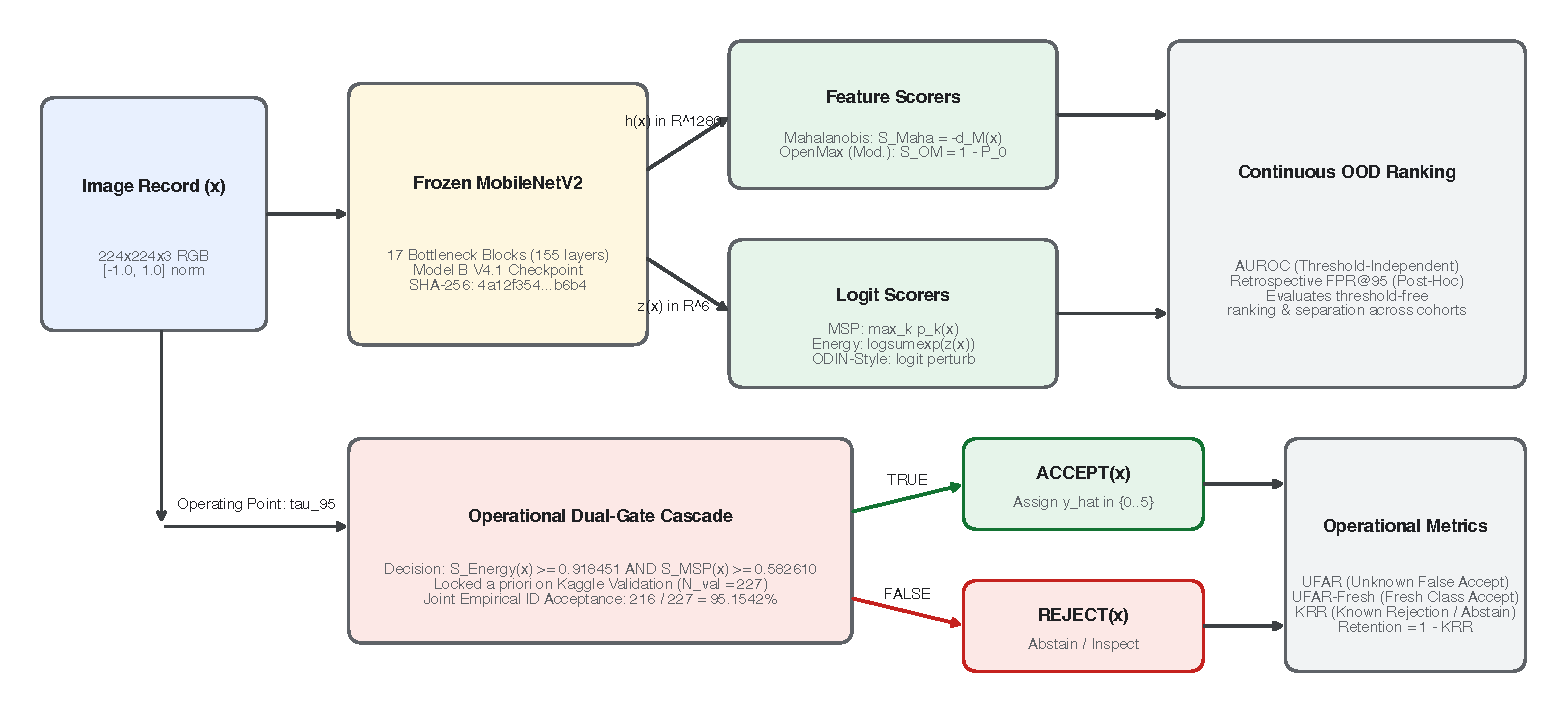
\includegraphics[width=0.98\linewidth]{figures/figure_02_pipeline.pdf}
\caption{End-to-end methodological pipeline of the source-stratified evaluation benchmark. Photographic image records are processed by a frozen MobileNetV2 backbone (checkpoint SHA-256: \texttt{4a12f354...b6b4}) to extract penultimate features $h(x) \in \mathbb{R}^{1280}$ and logits $z(x) \in \mathbb{R}^6$. Five post-hoc scoring functions are evaluated for continuous OOD ranking. Operating thresholds locked a priori on validation knowns ($N_{\text{val}} = 227$) govern discrete acceptance ($\hat{y} \in \{0, \dots, 5\}$) or rejection ($\hat{y} = \text{\textcircled{r}}$) via the Energy--MSP Dual-Gate cascade.}
\label{fig:methodological_pipeline}
\end{figure*}

\subsection{Frozen MobileNetV2 Classifier}
\label{sec:classifier_architecture}

The classification backbone is a lightweight convolutional neural network based on the MobileNetV2 architecture \cite{sandler2018mobilenetv2}, designed for resource-constrained edge execution.

\subsubsection{Architecture and Output Space}
The network comprises an initial $3 \times 3$ standard convolution followed by 17 bottleneck blocks: 1 initial inverted bottleneck stage without expansion and 16 inverted residual bottleneck blocks with depthwise separable convolutions and linear bottlenecks (expansion factor 6) \cite{sandler2018mobilenetv2}. In the Keras functional implementation, the feature extractor encompasses 155 layer operations terminating in a global average pooling layer that compresses spatial feature maps into a $D = 1280$ dimensional embedding $h(x) \in \mathbb{R}^{1280}$. The classification head consists of a dropout layer ($p = 0.3$) followed by a single fully connected dense layer parameterised by weight matrix $W \in \mathbb{R}^{1280 \times 6}$ and bias vector $b \in \mathbb{R}^6$:
\begin{equation}
z(x) = W^\top h(x) + b, \quad z(x) \in \mathbb{R}^6.
\end{equation}
The discrete target label space encompasses $K = 6$ commercial fruit freshness classes:
\begin{equation}
\begin{aligned}
\mathcal{Y} = \{ & 0: \text{fresh\_apple}, \; 1: \text{fresh\_banana}, \; 2: \text{fresh\_orange}, \\
                 & 3: \text{rotten\_apple}, \; 4: \text{rotten\_banana}, \; 5: \text{rotten\_orange} \}.
\end{aligned}
\end{equation}

\subsubsection{Model Provenance and Immutability Safeguards}
The evaluated model (designated Model B V4.1) was trained on $N_{\text{train}} = 9,513$ images from the primary Kaggle archive using AdamW optimization (initial learning rate $10^{-3}$, weight decay $10^{-4}$, label smoothing $\alpha = 0.05$) under group-aware partition separation. The final model checkpoint is stored as {\small\nolinkurl{MODEL_B_V4_1_CHECKPOINT.keras}} and verified by cryptographic checksum:
\begin{center}
\footnotesize
\texttt{SHA-256: 4a12f354a4157d2b04ed9606df7112c663fe000d924c5264b5f2fa1b3932b6b4}
\end{center}
Throughout all external evaluations across Partitions B, C, D1, and D2, this checkpoint remained strictly frozen (`\texttt{training=False}'). No weights, biases, batch normalization statistics, or hyperparameters were adjusted or fine-tuned.

\subsubsection{Input Preprocessing}
Input images of arbitrary resolution and aspect ratio are decoded from raw JPEG/PNG formats, resized to $(224, 224, 3)$ using bilinear interpolation, and converted to 32-bit floating-point tensors. Pixel intensities in $[0, 255]$ are normalized according to the standard MobileNetV2 mapping:
\begin{equation}
x_{\text{norm}} = \frac{x}{127.5} - 1.0 \in [-1.0, 1.0]^3.
\end{equation}

\subsection{Post-Hoc OOD Detection Scoring Functions}
\label{sec:ood_scoring_functions}

We evaluate five established post-hoc scoring algorithms, covering posterior probabilities, energy modeling, input perturbation, distance-based feature modeling, and extreme value theory. Table~\ref{tab:detector_formulations} summarizes their mathematical definitions, input representations, score orientations, and implementation hyperparameters.

\begin{table*}[!t]
\caption{Post-hoc out-of-distribution detector formulations and verified implementation configurations. All scores are oriented such that higher values indicate in-distribution confidence, ensuring consistency across continuous AUROC ranking and operational decision gating.}
\label{tab:detector_formulations}
\centering
\footnotesize
\setlength{\tabcolsep}{2.5pt}
\begin{tabular}{>{\raggedright\arraybackslash}p{1.8cm} >{\raggedright\arraybackslash}p{4.4cm} >{\centering\arraybackslash}p{1.8cm} >{\centering\arraybackslash}p{2.0cm} >{\raggedright\arraybackslash}p{4.2cm}}
\toprule
\textbf{Scoring Method} & \textbf{Mathematical Formulation} & \textbf{Input Layer} & \textbf{Score Direction} & \textbf{Verified Implementation Settings} \\
\midrule
\textbf{MSP} \newline Hendrycks \& Gimpel \cite{hendrycks2017baseline} & $S_{\text{MSP}}(x) = \max_{k} \frac{\exp(z_k(x))}{\sum_j \exp(z_j(x))}$ & Logits $z(x) \in \mathbb{R}^6$ & Higher $\implies$ ID \newline Anomaly: $-S_{\text{MSP}}$ & Standard softmax posterior; temperature $T = 1.0$; zero hyperparameter tuning. \\
\addlinespace[3pt]
\textbf{Energy} \newline Liu et al. \cite{liu2020energy} & $S_{\text{Energy}}(x) = T \cdot \log \sum_{k=1}^K \exp(z_k(x) / T)$ & Logits $z(x) \in \mathbb{R}^6$ & Higher $\implies$ ID \newline Anomaly: $-S_{\text{Energy}}$ & Free-energy score; temperature $T = 1.0$; computed via \texttt{logsumexp}. Post-hoc score, not generative density $p(x)$. \\
\addlinespace[3pt]
\textbf{ODIN (Variant)} \newline Liang et al. \cite{liang2018enhancing} & $S_{\text{ODIN}}(x) = \max_{k} \frac{\exp(z_k(\tilde{x}) / T)}{\sum_j \exp(z_j(\tilde{x}) / T)}$ \newline $\tilde{x} = \operatorname{clip}(x + \varepsilon \operatorname{sign}(\nabla_x \max_k z_k / T))$ & Image $x$ and logits $z(x)$ & Higher $\implies$ ID \newline Anomaly: $-S_{\text{ODIN}}$ & ODIN-style perturbation variant; gradient on max temperature-scaled logit; $T = 1000.0$; $\varepsilon = 0.0014$; clipped to $[-1.0, 1.0]$. \\
\addlinespace[3pt]
\textbf{Mahalanobis} \newline Lee et al. \cite{lee2018simple} & $S_{\text{Maha}}(x) = - \min_c d_M(h(x), \mu_c)$ \newline $d_M = \sqrt{(h(x) - \mu_c)^\top \Sigma_{\text{LW}}^{-1} (h(x) - \mu_c)}$ & Features $h(x) \in \mathbb{R}^{1280}$ & Higher $\implies$ ID \newline Anomaly: $d_M(x)$ & Class centroids $\mu_c$; shared covariance with Ledoit-Wolf shrinkage $\Sigma_{\text{LW}}$; negated distance. \\
\addlinespace[3pt]
\textbf{OpenMax (Mod.)} \newline Bendale \& Boult \cite{bendale2016towards} & $S_{\text{OpenMax}}(x) = 1.0 - p_{\text{OM}}(y = 0)$ \newline $w_{c_r} = 1.0 - \frac{r-1}{\alpha}(1 - \omega_r)$ & Features $h(x)$ and logits $z(x)$ & Higher $\implies$ ID \newline Anomaly: $p_{\text{OM}}(0) - 1$ & Modified OpenMax-style heuristic; 1280-D global pooled features; Weibull tail $\eta = 20$; $\alpha = 2$; rank weighting gives top-1 class zero logit discount. \\
\bottomrule
\end{tabular}
\end{table*}

\subsubsection{Maximum Softmax Probability (MSP)}
The baseline detector proposed by Hendrycks and Gimpel \cite{hendrycks2017baseline} computes the maximum posterior probability across known classes:
\begin{equation}
p_k(x) = \frac{\exp(z_k(x))}{\sum_{j=1}^K \exp(z_j(x))}, \quad S_{\text{MSP}}(x) = \max_{k \in \{0, \dots, K-1\}} p_k(x).
\end{equation}
Because softmax normalization enforces $\sum_k p_k(x) = 1$, the score $S_{\text{MSP}}(x) \in (1/K, 1]$ directly reflects the classifier's relative confidence. Higher MSP values indicate in-distribution confidence; lower values indicate uncertainty. For AUROC calculations where out-of-distribution instances represent the positive class ($y_{\text{ood}} = 1$), the anomaly ranking score is $-S_{\text{MSP}}(x)$.

\subsubsection{Energy-Based OOD Detection}
To overcome softmax probability saturation on anomalous inputs, Liu et al. \cite{liu2020energy} proposed an energy-based scoring function derived from the Helmholtz free energy. In physical systems, the free energy $E(x; f)$ is defined as $E(x; f) = -T \cdot \log \sum_k \exp(z_k(x) / T)$. In this study, to maintain mathematical consistency with the operational Dual-Gate acceptance equation ($S(x) \ge \tau$), we define the in-distribution energy score directly as the negative free energy (the log-sum-exp of logits):
\begin{equation}
S_{\text{Energy}}(x) = T \cdot \log \sum_{k=0}^{K-1} \exp\left(\frac{z_k(x)}{T}\right).
\end{equation}
In our implementation, the temperature is set to $T = 1.0$, simplifying the formulation to $S_{\text{Energy}}(x) = \operatorname{logsumexp}(z(x))$. Higher energy scores indicate larger unnormalized logit magnitudes and higher in-distribution confidence. We emphasize that $S_{\text{Energy}}(x)$ represents a post-hoc discriminator score, and is not claimed to represent an exact generative data density $p(x)$.

\subsubsection{ODIN-Style Perturbation Variant}
The ODIN framework proposed by Liang et al. \cite{liang2018enhancing} combines temperature scaling with adversarial input perturbation to enlarge score separation between in-distribution and anomalous inputs. In canonical ODIN, the input perturbation is derived from the gradient of the negative log temperature-scaled softmax probability of the predicted class: $-\log S_{\hat{y}}(x; T_{\text{ODIN}})$. In our canonical benchmark implementation ({\small\nolinkurl{scripts/run_stage4_1_benchmark.py}}), an ODIN-style perturbation variant is evaluated where the gradient target is the maximum temperature-scaled logit:
\begin{enumerate}
\item \textbf{Input Perturbation:} The input image is perturbed along the sign of the gradient of the maximum temperature-scaled logit:
\begin{equation}
x_{\text{perturbed}} = \operatorname{clip}\left( x + \varepsilon_{\text{ODIN}} \cdot \operatorname{sign}\left( \nabla_x \max_{k} \frac{z_k(x)}{T_{\text{ODIN}}} \right), \; -1.0, \; 1.0 \right).
\end{equation}
Because input imagery is preprocessed via the standard MobileNetV2 normalization mapping $x_{\text{norm}} \in [-1.0, 1.0]^3$, perturbed values are strictly clipped to the valid dynamic range $[-1.0, 1.0]$.
\item \textbf{Temperature-Scaled Confidence Scoring:} The perturbed image $x_{\text{perturbed}}$ is passed through the network, and the score is computed as the maximum temperature-scaled softmax probability:
\begin{equation}
S_{\text{ODIN}}(x) = \max_{k \in \{0, \dots, K-1\}} \frac{\exp(z_k(x_{\text{perturbed}}) / T_{\text{ODIN}})}{\sum_{j=0}^{K-1} \exp(z_j(x_{\text{perturbed}}) / T_{\text{ODIN}})}.
\end{equation}
\end{enumerate}
In our canonical implementation, hyperparameters are locked at $T_{\text{ODIN}} = 1000.0$ and $\varepsilon_{\text{ODIN}} = 0.0014$, verified against {\small\nolinkurl{scripts/run_stage4_1_benchmark.py}}. We explicitly document this implementation as an ODIN-style variant optimizing the top logit directly rather than canonical cross-entropy loss. Higher values denote in-distribution confidence.

\subsubsection{Mahalanobis Distance}
Following Lee et al. \cite{lee2018simple}, the Mahalanobis detector models penultimate feature representations using class-conditional Gaussian distributions with a tied covariance matrix.
\begin{enumerate}
\item \textbf{Centroid Estimation:} Using training features $h(x) \in \mathbb{R}^{1280}$, class mean vectors are computed as:
\begin{equation}
\mu_c = \frac{1}{N_c} \sum_{i : y_i = c} h(x_i), \quad c \in \{0, \dots, K-1\}.
\end{equation}
\item \textbf{Regularized Covariance Estimation:} To ensure invertibility and mitigate singularity in high-dimensional feature space ($D = 1280$), the shared covariance matrix is estimated using the Ledoit--Wolf shrinkage estimator on centered training features:
\begin{equation}
\Sigma_{\text{LW}} = (1 - \rho) \Sigma_{\text{sample}} + \rho \, \nu I_D,
\end{equation}
where $\rho \in [0, 1]$ is the analytically optimal shrinkage intensity and $\nu = \frac{1}{D} \operatorname{tr}(\Sigma_{\text{sample}})$.
\item \textbf{Score Formulation:} For test input $x$, the squared Mahalanobis distance to the closest class centroid is computed:
\begin{equation}
d_M^2(x) = \min_{c \in \{0, \dots, K-1\}} (h(x) - \mu_c)^\top \Sigma_{\text{LW}}^{-1} (h(x) - \mu_c).
\end{equation}
To maintain directional alignment with other detectors, the score is defined as the negated distance:
\begin{equation}
S_{\text{Maha}}(x) = - \sqrt{\max\left(d_M^2(x), 0\right)}.
\end{equation}
Higher values of $S_{\text{Maha}}(x)$ indicate closer proximity to training class clusters (in-distribution), whereas large negative values indicate anomalous outliers.
\end{enumerate}

\subsubsection{Modified OpenMax-Style Heuristic}
Bendale and Boult \cite{bendale2016towards} introduced OpenMax to calibrate classification logits using Extreme Value Theory (EVT) and estimate an explicit open-set unknown probability. In this study, the benchmark evaluates a modified OpenMax-style heuristic characterized by two implementation specifics:
\begin{enumerate}
\item \textbf{Feature Embedding Representation:} Class Mean Activation Vectors (MAVs) $\mu_c^{\text{MAV}} \in \mathbb{R}^{1280}$ and Euclidean distance modeling are evaluated on the 1280-dimensional global-average-pooled penultimate feature embedding $h(x) \in \mathbb{R}^{1280}$, rather than the multi-dimensional spatial activation tensors or layer-specific activation vectors of the original 2016 architecture.
\item \textbf{Weibull Tail Fitting:} For each class $c$, Euclidean distances $\|h(x_i) - \mu_c^{\text{MAV}}\|_2$ are computed over correctly classified training samples. A Weibull distribution $\operatorname{Weibull}(\text{shape}_c, \text{scale}_c)$ is fitted to the $\eta = 20$ largest distances (tail size $\eta = 20$, location parameter fixed at 0).
\item \textbf{Rank-Weighting Formulation and Deviation:} At inference, classes are ranked in descending order of logits $z_{(1)}(x) \ge z_{(2)}(x) \ge \dots \ge z_{(K)}(x)$. For the top $\alpha = 2$ ranked classes (with 1-based rank index $r \in \{1, \dots, \alpha\}$, corresponding to 0-based index $r-1$), the Weibull survival probability is evaluated:
\begin{equation}
\omega_r(x) = \exp\left( - \left( \frac{\|h(x) - \mu_{c_r}^{\text{MAV}}\|_2}{\text{scale}_{c_r} + 10^{-8}} \right)^{\text{shape}_{c_r}} \right).
\end{equation}
The logit adjustment weight implemented in the canonical codebase ({\small\nolinkurl{scripts/run_stage4_1_benchmark.py}}) is:
\begin{equation}
w_{c_r} = 1.0 - \frac{r - 1}{\alpha} (1.0 - \omega_r(x)),
\end{equation}
while unranked classes retain $w_k = 1.0$. Crucially, under this formulation, the highest-ranked class ($r = 1$) receives $\frac{1 - 1}{\alpha} = 0$, yielding $w_{c_1} = 1.0$ regardless of $\omega_1(x)$. Consequently, the top-1 predicted logit undergoes zero logit discounting, and Weibull probability recalibration affects only the second-ranked class ($r = 2$, receiving $w_{c_2} = 1.0 - 0.5(1.0 - \omega_2(x))$). This represents a distinct modified OpenMax-style heuristic compared to canonical OpenMax, where the top-ranked class receives the strongest Weibull tail calibration.
\item \textbf{Synthetic Unknown Class Softmax:} An augmented pseudo-logit for the unknown class (index 0) is constructed as:
\begin{equation}
\hat{v}_0(x) = \sum_{k=0}^{K-1} z_k(x) (1.0 - w_k), \quad \hat{v}_{k+1}(x) = z_k(x) \cdot w_k.
\end{equation}
Applying softmax across the resulting $K+1$ logits produces posterior probability vector $p_{\text{OM}} \in \Delta^K$. The in-distribution confidence score is defined as:
\begin{equation}
S_{\text{OpenMax}}(x) = 1.0 - p_{\text{OpenMax}}(y = 0).
\end{equation}
Higher values indicate that the produce belongs to one of the six known classes; lower values reflect high open-set unknown probability.
\end{enumerate}

\subsection{Operational Energy--MSP Dual-Gate Cascade}
\label{sec:dualgate_cascade}

In agricultural packaging and sorting operations, continuous anomaly scores must be converted into deterministic routing decisions: either accepting the produce item for automated packaging under the classifier's top-1 predicted label, or rejecting the item to an abstention bin for manual inspection.

\subsubsection{Motivation and Cascade Formulation}
Empirical analysis reveals that standalone detectors exhibit complementary failure modes: Energy scores capture unnormalized activation magnitude and separate coarse semantic out-of-distribution produce, whereas MSP reflects posterior distribution peakedness and discriminates ambiguous in-distribution boundaries. The Dual-Gate cascade integrates both criteria into an operational decision heuristic.

We emphasize that the Dual-Gate cascade is an \textit{operational decision rule}, not a novel standalone mathematical model or learning algorithm. For any incoming image $x$, the discrete acceptance decision is defined as:
\begin{equation}
\label{eq:dualgate_rule}
\operatorname{ACCEPT}(x) \iff S_{\text{Energy}}(x) \ge \tau_E \;\land\; S_{\text{MSP}}(x) \ge \tau_M.
\end{equation}
Otherwise:
\begin{equation}
\operatorname{REJECT}(x) \iff S_{\text{Energy}}(x) < \tau_E \;\lor\; S_{\text{MSP}}(x) < \tau_M.
\end{equation}
When $\operatorname{ACCEPT}(x) = 1$, the model assigns its closed-set predicted class:
\begin{equation}
\hat{y}(x) = \arg\max_{k \in \{0, \dots, 5\}} z_k(x).
\end{equation}
When $\operatorname{REJECT}(x) = 1$, the system abstains from classification and routes the image record to manual review ($\hat{y}(x) = \text{\textcircled{r}}$).

\subsubsection{Continuous Margin Proxy for Exploratory AUROC}
Because the Dual-Gate rule evaluates a Boolean conjunction ($g_E(x) \land g_M(x)$), it produces a discrete binary decision ($\{0, 1\}$) rather than a continuous ranking score, and therefore cannot directly generate an ROC curve without a continuous ranking proxy. To permit exploratory comparative ROC analysis in benchmark tables, we compute a continuous linear margin proxy:
\begin{equation}
S_{\text{proxy}}(x) = (S_{\text{Energy}}(x) - \tau_E) + (S_{\text{MSP}}(x) - \tau_M).
\end{equation}
We emphasize that this continuous linear margin proxy is strictly an exploratory metric. Because raw Energy scores (log-sum-exp of logits, typical range $[0, 10]$) and MSP scores (posterior probabilities in $(1/6, 1]$) reside on substantially different numerical scales, this unweighted additive combination is inherently scale-dependent and dominated by Energy variations. The proxy does not constitute a canonical continuous score of the Dual-Gate. All operational routing and acceptance metrics (UFAR, UFAR-Fresh, KRR, Retention) are evaluated strictly using the exact discrete Boolean conjunction in Eq.~\eqref{eq:dualgate_rule}.

\subsection{Validation-Based Operating-Threshold Calibration}
\label{sec:threshold_calibration}

To reduce potential circularity and data-snooping bias, all operating thresholds were calibrated strictly on an independent primary validation partition and locked prior to external evaluation.

\subsubsection{Calibration Population}
The calibration population comprises $N_{\text{val}} = 227$ raw photographic images from the primary Kaggle validation split ({\small\nolinkurl{FINAL_GROUP_VAL_V4_1.csv}}, filtered by `\texttt{is\_raw == 1}'). This set contains 35 fresh apples, 49 rotten apples, 33 fresh bananas, 46 rotten bananas, 31 fresh oranges, and 33 rotten oranges. As established in Section~\ref{sec:evaluation_integrity}, MD5 cryptographic hashing confirms zero file overlap with the 227-image test set (Partition A), and the 227 validation images are completely excluded from the 13,465-image evaluation census.

\subsubsection{Order-Statistic Calibration Protocol}
Thresholds were derived using non-parametric empirical order statistics to target approximately 95\% in-distribution acceptance coverage ($\tau_{95}$, corresponding to an empirical false rejection / abstention budget of $\le 5.0\%$). Table~\ref{tab:threshold_calibration} details the exact calibration parameters, order-statistic indices, and empirical validation coverage for each configuration.

\begin{table*}[!t]
\caption{Validation-based operating threshold calibration on primary validation data ($N_{\text{val}} = 227$ raw images). All thresholds were locked a priori using empirical order statistics and held fixed throughout external evaluations. Dual-Gate thresholds are jointly calibrated to account for rejection overlap, achieving matched 95.1542\% empirical in-distribution coverage.}
\label{tab:threshold_calibration}
\centering
\footnotesize
\setlength{\tabcolsep}{2.5pt}
\begin{tabular}{>{\raggedright\arraybackslash}p{2.2cm} >{\centering\arraybackslash}p{1.5cm} >{\centering\arraybackslash}p{1.6cm} >{\centering\arraybackslash}p{1.8cm} >{\centering\arraybackslash}p{2.1cm} >{\centering\arraybackslash}p{1.6cm} >{\raggedright\arraybackslash}p{3.0cm}}
\toprule
\textbf{Configuration / Detector} & \textbf{Score Symbol} & \textbf{Locked Threshold ($\tau_{95}$)} & \textbf{Order-Statistic Index ($s_{(k)}$)} & \textbf{Validation Rejected / Accepted} & \textbf{Empirical ID Coverage} & \textbf{Operational Comparison Rule} \\
\midrule
\textbf{MSP (Single Gate)} & $S_{\text{MSP}}$ & 0.700580 & 12th smallest $s_{(12)}$ (index 11) & 11 rejected / 216 accepted & 95.1542\% & $\operatorname{ACCEPT} \iff$ \newline $S_{\text{MSP}} \ge 0.700580$ \\
\addlinespace[3pt]
\textbf{Energy (Single Gate)} & $S_{\text{Energy}}$ & 1.054579 & 12th smallest $s_{(12)}$ (index 11) & 11 rejected / 216 accepted & 95.1542\% & $\operatorname{ACCEPT} \iff$ \newline $S_{\text{Energy}} \ge 1.054579$ \\
\addlinespace[3pt]
\textbf{ODIN (Single Gate)} & $S_{\text{ODIN}}$ & 0.167164 & 12th smallest $s_{(12)}$ (index 11) & 11 rejected / 216 accepted & 95.1542\% & $\operatorname{ACCEPT} \iff$ \newline $S_{\text{ODIN}} \ge 0.167164$ \\
\addlinespace[3pt]
\textbf{Mahalanobis (Single Gate)} & $S_{\text{Maha}}$ & -65.133230 & 12th smallest $s_{(12)}$ (index 11) & 11 rejected / 216 accepted & 95.1542\% & $\operatorname{ACCEPT} \iff$ \newline $S_{\text{Maha}} \ge -65.133230$ \\
\addlinespace[3pt]
\textbf{OpenMax (Single Gate)} & $S_{\text{OpenMax}}$ & 0.778938 & 12th smallest $s_{(12)}$ (index 11) & 11 rejected / 216 accepted & 95.1542\% & $\operatorname{ACCEPT} \iff$ \newline $S_{\text{OpenMax}} \ge 0.778938$ \\
\midrule
\textbf{Dual-Gate Cascade} \newline (Energy AND MSP) & $\tau_E \text{ and } \tau_M$ & $\tau_E = 0.918451$ \newline $\tau_M = 0.582610$ & 7th smallest $s_{(7)}$ (index 6) on both scores & $|R_1|=6, |R_2|=6$ \newline $|R_1 \cap R_2|=1 \implies$ 11 rejected / 216 accepted & 95.1542\% & $\operatorname{ACCEPT} \iff$ \newline $S_{\text{Energy}} \ge 0.918451 \;\land$ \newline $S_{\text{MSP}} \ge 0.582610$ \\
\bottomrule
\end{tabular}
\end{table*}

\begin{enumerate}
\item \textbf{Standalone Single-Gate Thresholds:} Let $\{s_{(1)} \le s_{(2)} \le \dots \le s_{(N_{\text{val}})}\}$ denote the sorted validation scores of a detector. Selecting the 12th smallest order statistic ($s_{(12)}$, 0-indexed position 11) establishes a threshold that rejects the 11 smallest scores ($S < s_{(12)}$) and accepts the remaining $227 - 11 = 216$ samples:
\begin{equation}
\text{Empirical In-Distribution Coverage} = \frac{216}{227} \approx 95.1542\%.
\end{equation}
Under this rule, standalone Energy yields $\tau_{\text{Energy}} = 1.054579$ and standalone MSP yields $\tau_{\text{MSP}} = 0.700580$.
\item \textbf{Joint Dual-Gate Calibration via Inclusion--Exclusion:} If the standalone thresholds were applied simultaneously in an AND-rule, rejections would compound: $|R_{\text{union}}| = |R_E \cup R_M| > 11$, reducing in-distribution acceptance far below 95\%. To maintain matched $95.1542\%$ empirical coverage, the thresholds for both gates are jointly calibrated using empirical set intersection:
\begin{itemize}
\item Gate 1 (Energy) threshold is relaxed to the 7th smallest order statistic ($s_{(7)}$, index 6): $\tau_E = 0.918451$, rejecting $|R_1| = 6$ samples.
\item Gate 2 (MSP) threshold is relaxed to the 7th smallest order statistic ($s_{(7)}$, index 6): $\tau_M = 0.582610$, rejecting $|R_2| = 6$ samples.
\item Exactly 1 sample falls below both thresholds simultaneously: $|R_1 \cap R_2| = 1$.
\item By the inclusion--exclusion principle, the total number of rejected validation samples is:
\begin{equation}
|R_{\text{union}}| = |R_1| + |R_2| - |R_1 \cap R_2| = 6 + 6 - 1 = 11.
\end{equation}
\item The joint in-distribution acceptance count is exactly $227 - 11 = 216$, matching the canonical $95.1542\%$ empirical validation coverage.
\end{itemize}
\end{enumerate}

We emphasize that the observed $95.1542\%$ validation coverage represents an empirical sample proportion, not a guaranteed population-level coverage certificate; with $N_{\text{val}} = 227$, the 95\% Clopper--Pearson exact binomial interval spans $[91.43\%, 97.60\%]$.

\subsection{Evaluation Metrics}
\label{sec:evaluation_metrics}

To evaluate model performance across multiple operational dimensions, we define three categories of metrics, summarized in Table~\ref{tab:metric_definitions}.

\begin{table*}[!t]
\caption{Authoritative evaluation metrics, mathematical formulations, target directions, and operational evaluation scopes across closed-set classification, continuous out-of-distribution ranking, and operational rejection gating.}
\label{tab:metric_definitions}
\centering
\footnotesize
\setlength{\tabcolsep}{2.5pt}
\begin{tabular}{>{\raggedright\arraybackslash}p{2.2cm} >{\centering\arraybackslash}p{2.0cm} >{\raggedright\arraybackslash}p{4.4cm} >{\centering\arraybackslash}p{1.4cm} >{\raggedright\arraybackslash}p{4.3cm}}
\toprule
\textbf{Metric Name} & \textbf{Category} & \textbf{Mathematical Formulation} & \textbf{Target Direction} & \textbf{Operational Scope and Meaning} \\
\midrule
\textbf{Top-1 Accuracy} & Closed-Set Classification & $\text{Acc} = \frac{1}{N} \sum_{i=1}^N \mathbf{1}\{\hat{y}_i = y_i\}$ & Higher ($\uparrow$) & Overall proportion of correct predictions across known classes $\mathcal{Y}$. \\
\addlinespace[3pt]
\textbf{Balanced Accuracy} & Closed-Set Classification & $\text{BalAcc} = \frac{1}{K} \sum_{k=0}^{K-1} \frac{\text{TP}_k}{N_k}$ & Higher ($\uparrow$) & Unweighted macro-averaged recall across all 6 known classes; eliminates class-imbalance bias. \\
\addlinespace[3pt]
\textbf{Macro-Averaged F1} & Closed-Set Classification & $\text{Macro-F1} = \frac{1}{K} \sum_{k=0}^{K-1} \frac{2 P_k R_k}{P_k + R_k}$ & Higher ($\uparrow$) & Harmonic mean of class-wise precision and recall; treats all 6 target classes with equal weight. \\
\midrule
\textbf{AUROC} & Continuous OOD Ranking & $\text{AUROC} = \int_{0}^1 \text{TPR}(\tau) \, d(\text{FPR}(\tau))$ & Higher ($\uparrow$) & Area under ROC curve treating OOD as positive ($y_{\text{ood}} = 1$); threshold-independent ranking. \\
\addlinespace[3pt]
\textbf{Retrospective FPR@95} & Retrospective OOD Separation & $\text{FPR@95} = \frac{|\{x \in \mathcal{D}_{\text{ood}} : S(x) \ge \tau_{95}^{\text{test}}\}|}{|\mathcal{D}_{\text{ood}}|}$ & Lower ($\downarrow$) & False positive rate on OOD when $\tau_{95}^{\text{test}}$ fixes ID TPR at 95.0\%; retrospective operating-point metric, not threshold-independent. \\
\addlinespace[3pt]
\textbf{OSCR} & Open-Set Classification & $\text{OSCR} = \int_{0}^1 \text{CCR}(\tau) \, d(\text{FPR}(\tau))$ & Higher ($\uparrow$) & Area under Correct Classification Rate vs. False Positive Rate curve. \\
\midrule
\textbf{Operational UFAR} & Operational Rejection Gating & $\text{UFAR}(\tau_{95}) = \frac{|\{x \in \mathcal{D}_{\text{ood}} : \operatorname{ACCEPT}(x)\}|}{|\mathcal{D}_{\text{ood}}|}$ & Lower ($\downarrow$) & Proportion of out-of-distribution image records accepted under fixed validation threshold $\tau_{95}$. \\
\addlinespace[3pt]
\textbf{Operational UFAR-Fresh} & Produce Routing Outcome & $\text{UFAR-F}(\tau_{95}) = \frac{|\{x \in \mathcal{D}_{\text{ood}} : \operatorname{ACCEPT}(x) \land \hat{y}(x) \in \text{Fresh}\}|}{|\mathcal{D}_{\text{ood}}|}$ & Lower ($\downarrow$) & Proportion of OOD images accepted and assigned to a commercial Fresh class; image-level non-target acceptance outcome, not verified biological food safety. \\
\addlinespace[3pt]
\textbf{Operational KRR} \newline (Abstention Rate) & Operational Inspection Cost & $\text{KRR}(\tau_{95}) = \frac{|\{x \in \mathcal{D}_{\text{id}} : \operatorname{REJECT}(x)\}|}{|\mathcal{D}_{\text{id}}|}$ & Lower ($\downarrow$) & Known-class rejection rate: proportion of valid known images unnecessarily routed to manual inspection. \\
\addlinespace[3pt]
\textbf{Known Retention} & Operational Automation & $\text{Retention} = 1 - \text{KRR}(\tau_{95})$ & Higher ($\uparrow$) & Proportion of valid commercial known images retained and classified automatically without human review. \\
\bottomrule
\end{tabular}
\end{table*}

\subsubsection{Closed-Set Classification Metrics}
Evaluated strictly on known-class partitions (Partition A, $N = 227$; Partition B, $N = 5,350$):
\begin{enumerate}
\item \textbf{Top-1 Accuracy:} $\text{Acc} = \frac{1}{N} \sum_{i=1}^N \mathbf{1}\{\hat{y}_i = y_i\}$.
\item \textbf{Balanced Accuracy:} Arithmetic mean of recall across all $K = 6$ classes, preventing majority-class dominance:
\begin{equation}
\text{Balanced Accuracy} = \frac{1}{K} \sum_{k=0}^{K-1} \frac{\text{TP}_k}{N_k}.
\end{equation}
\item \textbf{Macro-Averaged F1:} Unweighted average of class-wise F1 scores:
\begin{equation}
\text{Macro-F1} = \frac{1}{K} \sum_{k=0}^{K-1} \frac{2 \cdot \text{Precision}_k \cdot \text{Recall}_k}{\text{Precision}_k + \text{Recall}_k}.
\end{equation}
\end{enumerate}

\subsubsection{Continuous Out-of-Distribution Discrimination Metrics}
Evaluated across in-distribution and out-of-distribution subsets ($\mathcal{D}_{\text{id}} \cup \mathcal{D}_{\text{ood}}$):
\begin{enumerate}
\item \textbf{Area Under the ROC Curve (AUROC):} Measures threshold-independent pairwise ranking capability. In our evaluation protocol, out-of-distribution instances represent the positive class ($y_{\text{ood}} = 1$) and in-distribution known instances represent the negative class ($y_{\text{id}} = 0$). With detector score $S(x)$ oriented such that higher values denote in-distribution, the anomaly score is defined as $-S(x)$. The AUROC equals the probability that a randomly drawn OOD sample receives a higher anomaly score than a randomly drawn ID sample:
\begin{equation}
\text{AUROC} = P(-S(x_{\text{ood}}) > -S(x_{\text{id}})) = P(S(x_{\text{id}}) > S(x_{\text{ood}})).
\end{equation}
\item \textbf{Retrospective FPR@95:} The false positive rate (proportion of OOD images incorrectly accepted as known) when a threshold $\tau_{95}^{\text{test}}$ is chosen post-hoc on the evaluated test set to achieve exactly 95.0\% true positive rate (known retention) on $\mathcal{D}_{\text{id}}$:
\begin{equation}
\tau_{95}^{\text{test}} = \sup \left\{ \tau : \frac{|\{x \in \mathcal{D}_{\text{id}} : S(x) \ge \tau\}|}{|\mathcal{D}_{\text{id}}|} \ge 0.95 \right\}, \quad \text{FPR@95} = \frac{|\{x \in \mathcal{D}_{\text{ood}} : S(x) \ge \tau_{95}^{\text{test}}\}|}{|\mathcal{D}_{\text{ood}}|}.
\end{equation}
Unlike AUROC, FPR@95 evaluates separation specifically at a high-coverage operating point, but remains a retrospective metric tuned to the test partition, with out-of-distribution instances designated as the positive class ($y_{\text{ood}} = 1$).
\item \textbf{Auxiliary Open-Set Discrimination Metrics:} In addition to primary ranking and separation metrics, exploratory discrimination diagnostics were evaluated during execution: the Correct Classification Rate vs. False Positive Rate curve ($\text{OSCR} = \int_0^1 \text{CCR}(\tau) \, d(\text{FPR}(\tau))$) and precision-recall curves (AUPR-IN treating knowns as positive; AUPR-OUT treating OOD as positive), preserved in {\small\nolinkurl{STAGE4_1_2_SOURCE_STRATIFIED_METRICS.csv}}.
\end{enumerate}

\subsubsection{Operational Decision Metrics under Locked Validation Thresholds}
Evaluated strictly using the prospective thresholds ($\tau_{95}$) locked on the Kaggle validation set:
\begin{enumerate}
\item \textbf{Unknown False Acceptance Rate (UFAR):} The proportion of out-of-distribution image records accepted as known:
\begin{equation}
\text{UFAR}(\tau_{95}) = \frac{|\{x \in \mathcal{D}_{\text{ood}} : \operatorname{ACCEPT}(x)\}|}{|\mathcal{D}_{\text{ood}}|}.
\end{equation}
\item \textbf{Unknown-to-Fresh False Acceptance Rate (UFAR-Fresh):} The proportion of out-of-distribution image records accepted and specifically assigned to a commercial Fresh class ($\hat{y}(x) \in \{0, 1, 2\}$, corresponding to fresh apple, fresh banana, or fresh orange):
\begin{equation}
\text{UFAR-Fresh}(\tau_{95}) = \frac{|\{x \in \mathcal{D}_{\text{ood}} : \operatorname{ACCEPT}(x) \;\land\; \hat{y}(x) \in \{0, 1, 2\}\}|}{|\mathcal{D}_{\text{ood}}|}.
\end{equation}
Crucially, the denominator of UFAR-Fresh is the total number of OOD images ($|\mathcal{D}_{\text{ood}}|$), not the accepted subset, providing an absolute failure rate across the evaluated cohort. We reframe UFAR-Fresh strictly as an image-level sorting outcome representing acceptance and assignment to a Fresh known class; it is not claimed to represent verified biological food safety or commercial quality assurance certification.
\item \textbf{Known-Class Rejection Rate (KRR / Abstention Rate):} The proportion of valid known-class images rejected by the gate:
\begin{equation}
\text{KRR}(\tau_{95}) = \frac{|\{x \in \mathcal{D}_{\text{id}} : \operatorname{REJECT}(x)\}|}{|\mathcal{D}_{\text{id}}|}.
\end{equation}
\item \textbf{Known-Class Retention Rate:} The proportion of known produce retained for automated sorting: $\text{Retention} = 1 - \text{KRR}(\tau_{95})$.
\end{enumerate}

\subsection{Uncertainty Quantification and Statistical Reporting}
\label{sec:uncertainty_quantification}

All reported confidence intervals and statistical tests adhere to pre-specified, non-parametric protocols:
\begin{enumerate}
\item \textbf{Non-Parametric Bootstrap Protocol:} Point estimates are accompanied by 95\% bootstrap confidence intervals generated via $B = 1,000$ resamples with replacement. To ensure exact computational reproducibility, pseudo-random number generation was seeded at `\texttt{seed=42}'. Confidence intervals are constructed using the empirical percentile method:
\begin{equation}
\text{CI}_{95} = \left[ \hat{\theta}^*_{(0.025 \cdot B)}, \; \hat{\theta}^*_{(0.975 \cdot B)} \right] = \left[ \hat{\theta}^*_{(25)}, \; \hat{\theta}^*_{(975)} \right].
\end{equation}
\item \textbf{Resampling Unit and Stratification Strategy:} The resampling unit is strictly an \textit{individual image record}. For closed-set metrics on Partitions A and B, bootstrap resampling is stratified by the $K = 6$ known classes. For out-of-distribution cohort evaluations (Cohorts A--D), resampling is stratified jointly across the reference ID population and the OOD cohort by species and condition labels.
\item \textbf{Methodological Conditioning and Statistical Non-Independence:} All bootstrap confidence intervals are conditional on image-level exchangeability. As detailed in Section~\ref{sec:duplicate_handling_phash}, photographic records from web archives cannot be assumed to represent statistically independent biological fruit specimens. Furthermore, because FruitVision Known (Partition B, $N_{\text{id}} = 4,157$) is evaluated across Cohorts A, B, and C, the resulting confidence intervals across cohorts share a common reference population and must not be interpreted as statistically independent replications.
\item \textbf{Descriptive Comparison of Closed-Set Performance Differences:} The observed 28.56 percentage-point difference in top-1 accuracy between Partition A ($96.92\%$ [94.71\%, 98.68\%]) and Partition B ($68.36\%$ [67.20\%, 69.40\%]) displays non-overlapping 95\% bootstrap percentile intervals, reflecting substantial descriptive separation under the evaluated image-level resampling protocol without asserting formal inferential hypothesis testing.
\end{enumerate}

\subsection{Software and Implementation Reproducibility}
\label{sec:software_environment}

To ensure complete computational traceability, all experimental code was executed within a controlled software environment:
\begin{itemize}
\item \textbf{Software Stack:} Python 3.10.12, TensorFlow 2.15.0, Keras 3.0.5, NumPy 1.26.4, SciPy 1.13.0, scikit-learn 1.4.1.post1, and pandas 2.2.1.
\item \textbf{Image Processing Pipeline:} Standardized via {\small\nolinkurl{tf.io.decode_image}}, {\small\nolinkurl{tf.image.resize}} (bilinear), and {\small\nolinkurl{tf.keras.applications.mobilenet_v2.preprocess_input}}.
\item \textbf{OOD Implementation Libraries:} SciPy {\small\nolinkurl{scipy.special.logsumexp}} for Energy calculation; SciPy {\small\nolinkurl{scipy.stats.weibull_min}} for OpenMax Weibull tail fitting; scikit-learn Ledoit--Wolf shrinkage covariance estimation for Mahalanobis scoring; and TensorFlow {\small\nolinkurl{tf.GradientTape}} for ODIN input perturbations.
\item \textbf{Canonical Deliverable Ledgers:} Execution outputs are preserved in structured files within the repository root:
\begin{itemize}
\item Master image-level prediction and score table: \newline {\small\nolinkurl{STAGE4_1_IMAGE_LEVEL_PREDICTIONS.csv}}
\item Frozen validation operating thresholds: \newline {\small\nolinkurl{STAGE4_0_3_CORRECTED_THRESHOLD_TABLE.csv}}
\item Source-stratified point estimates: \newline {\small\nolinkurl{STAGE4_1_2_SOURCE_STRATIFIED_METRICS.csv}}
\item Authoritative bootstrap confidence intervals ($B = 1,000$): \newline {\small\nolinkurl{STAGE4_1_2_1_SOURCE_STRATIFIED_CONFIDENCE_INTERVALS.csv}}
\item Perceptual hash sensitivity evaluation tiers: \newline {\small\nolinkurl{STAGE4_1_2_1_SOURCE_STRATIFIED_PHASH_SENSITIVITY.csv}}
\item Final claims and evidence ledger: \newline {\small\nolinkurl{STAGE4_1_2_1_1_FINAL_CLAIMS_LEDGER.csv}}
\end{itemize}
\item \textbf{External Dependencies:} Full end-to-end re-execution requires access to the original photographic files distributed by Kaggle, FruitVision \cite{bijoy2025fruitvision}, and Sultana et al. \cite{sultana2022extensive} under their respective publisher terms.
\end{itemize}
\section{Experimental Results and Failure Analysis}
\label{sec:results}

This section presents the closed-set performance evaluation across partitions, source-stratified OOD detection AUROC and FPR@95 metrics, operational Dual-Gate rejection rates (UFAR, UFAR-Fresh, KRR), non-parametric bootstrap confidence intervals, and sensitivity analysis across perceptual-hash (pHash) near-duplicate exclusion tiers.

\subsection{Sensitivity and Near-Duplicate Robustness Analysis}
\label{sec:results_sensitivity}

To evaluate whether near-duplicate captures within external photographic archives artificially inflate or distort out-of-distribution detection metrics, detector performance was benchmarked across the three sensitivity tiers defined in Section~\ref{sec:duplicate_handling_phash}: Primary ($N = 13,465$), Tier 1 ($N = 13,409$), and Tier 2 ($N = 13,382$). Table~\ref{tab:phash_sensitivity} reports the complete empirical sensitivity evaluation across all five post-hoc scoring functions and the Dual-Gate operational decision rule for all four source-matched cohorts.

\begin{table*}[!t]
\caption{Sensitivity analysis of out-of-distribution detection performance (AUROC, \%) across perceptual-hash (pHash) near-duplicate exclusion tiers. Results cover all five post-hoc scoring functions and the exploratory Dual-Gate linear margin proxy across Cohorts A--D. Relative detector rankings remain strictly invariant across all three tiers within every evaluation cohort.}
\label{tab:phash_sensitivity}
\centering
\footnotesize
\setlength{\tabcolsep}{3.5pt}
\begin{tabular}{>{\raggedright\arraybackslash}p{3.8cm} >{\raggedright\arraybackslash}p{2.3cm} >{\centering\arraybackslash}p{2.0cm} >{\centering\arraybackslash}p{2.0cm} >{\centering\arraybackslash}p{2.0cm} >{\centering\arraybackslash}p{1.7cm}}
\toprule
\textbf{Evaluation Cohort} & \textbf{Scoring Function} & \textbf{Primary ($N=13,465$)} & \textbf{Tier 1 ($N=13,409$)} & \textbf{Tier 2 ($N=13,382$)} & \textbf{Max $|\Delta|$ (pp)} \\
\midrule
\textbf{Cohort A: Semantic Shift} & MSP & 72.42 & 72.38 & 72.33 & 0.09 \\
\textit{FruitVision B vs D1} & Energy & 81.57 & 81.53 & 81.46 & 0.11 \\
($N_{\text{id}} = 4,157$, & ODIN & 72.30 & 72.27 & 72.20 & 0.10 \\
$N_{\text{ood}} = 2,776 \to 2,746$) & Mahalanobis & 81.41 & 81.34 & 81.27 & 0.14 \\
 & OpenMax & 72.46 & 72.44 & 72.38 & 0.08 \\
 & Dual-Gate (Proxy) & 80.93 & 80.89 & 80.82 & 0.11 \\
\midrule
\textbf{Cohort B: Treatment Shift} & MSP & 58.77 & 58.80 & 58.81 & 0.04 \\
\textit{FruitVision B vs C} & Energy & 53.13 & 53.18 & 53.19 & 0.06 \\
($N_{\text{id}} = 4,157$, & ODIN & 56.73 & 56.78 & 56.78 & 0.05 \\
$N_{\text{ood}} = 1,917 \to 1,901$) & Mahalanobis & 47.91 & 47.96 & 48.01 & 0.10 \\
 & OpenMax & 55.35 & 55.38 & 55.40 & 0.05 \\
 & Dual-Gate (Proxy) & 53.96 & 54.01 & 54.02 & 0.06 \\
\midrule
\textbf{Cohort C: Combined Shift} & MSP & 76.47 & 76.48 & 76.50 & 0.03 \\
\textit{FruitVision B vs D2} & Energy & 84.72 & 84.64 & 84.65 & 0.08 \\
($N_{\text{id}} = 4,157$, & ODIN & 78.11 & 78.11 & 78.13 & 0.02 \\
$N_{\text{ood}} = 1,195 \to 1,175$) & Mahalanobis & 80.08 & 79.88 & 79.86 & 0.22 \\
 & OpenMax & 77.22 & 77.22 & 77.22 & 0.00 \\
 & Dual-Gate (Proxy) & 84.16 & 84.09 & 84.10 & 0.07 \\
\midrule
\textbf{Cohort D: Semantic Shift} & MSP & 59.77 & 59.77 & 59.77 & 0.00 \\
\textit{Sultana B vs D1} & Energy & 67.52 & 67.52 & 67.52 & 0.00 \\
($N_{\text{id}} = 1,193$, & ODIN & 60.02 & 60.02 & 60.02 & 0.00 \\
$N_{\text{ood}} = 2,000 \to 2,000$) & Mahalanobis & 68.15 & 68.15 & 68.15 & 0.00 \\
 & OpenMax & 64.38 & 64.38 & 64.38 & 0.00 \\
 & Dual-Gate (Proxy) & 66.68 & 66.68 & 66.68 & 0.00 \\
\bottomrule
\end{tabular}
\end{table*}

The sensitivity analysis demonstrates two critical empirical findings:
\begin{enumerate}
\item \textbf{High Metric Stability:} Across all 24 evaluated detector-cohort configurations, metric fluctuations between the Primary benchmark and Tier 2 remain minor: the maximum observed change in AUROC across all methods is $0.22$ percentage points (Mahalanobis in Cohort C, shifting from 80.08\% to 79.86\%). For most scoring functions, AUROC shifts are bounded within $\pm 0.11$ percentage points. In Cohort D (Sultana et al.), where zero cross-partition or multi-label pHash collisions were detected at $r \le 8$, metrics remain completely invariant.
\item \textbf{Strict Detector Ranking Invariance:} In all four cohorts, the relative ranking of detection methods is preserved without a single rank inversion across the three evaluation tiers:
\begin{itemize}
\item \textit{Cohort A (FruitVision Semantic Shift):} Energy (81.57\% $\to$ 81.46\%) $>$ Mahalanobis (81.41\% $\to$ 81.27\%) $>$ Dual-Gate Proxy (80.93\% $\to$ 80.82\%) $>$ OpenMax (72.46\% $\to$ 72.38\%) $>$ MSP (72.42\% $\to$ 72.33\%) $>$ ODIN (72.30\% $\to$ 72.20\%).
\item \textit{Cohort B (FruitVision Treatment Shift):} MSP (58.77\% $\to$ 58.81\%) $>$ ODIN (56.73\% $\to$ 56.78\%) $>$ OpenMax (55.35\% $\to$ 55.40\%) $>$ Dual-Gate Proxy (53.96\% $\to$ 54.02\%) $>$ Energy (53.13\% $\to$ 53.19\%) $>$ Mahalanobis (47.91\% $\to$ 48.01\%).
\item \textit{Cohort C (FruitVision Combined Shift):} Energy (84.72\% $\to$ 84.65\%) $>$ Dual-Gate Proxy (84.16\% $\to$ 84.10\%) $>$ Mahalanobis (80.08\% $\to$ 79.86\%) $>$ ODIN (78.11\% $\to$ 78.13\%) $>$ OpenMax (77.22\% $\to$ 77.22\%) $>$ MSP (76.47\% $\to$ 76.50\%).
\item \textit{Cohort D (Sultana Semantic Shift):} Mahalanobis (68.15\%) $>$ Energy (67.52\%) $>$ Dual-Gate Proxy (66.68\%) $>$ OpenMax (64.38\%) $>$ ODIN (60.02\%) $>$ MSP (59.77\%) (invariant across all three tiers).
\end{itemize}
\end{enumerate}

\noindent \textit{Evidence Bounds on Sensitivity Conclusions:} These results establish that the benchmark performance estimates and comparative method orderings are robust with respect to the tested pHash collision exclusions and evaluated image records. However, we qualify this conclusion: perceptual hashing at low-frequency DCT resolution captures detectable visual near-duplicates, but cannot prove the complete absence of subtle burst captures, viewpoint variations, or unmodelled specimen-level correlations in the underlying repositories. Complete point estimates and operational metrics across all tiers are preserved in canonical register: \newline {\raggedright\small\nolinkurl{STAGE4_1_2_1_SOURCE_STRATIFIED_PHASH_SENSITIVITY.csv}\par}
\section{Discussion}
\label{sec:discussion}

This section discusses the implications of external domain collapse, the visual limitations of RGB imaging for detecting chemical immersion protocols, and practical design recommendations for integrating secondary multi-modal sensor streams into agricultural grading pipelines.


\enlargethispage{\baselineskip}
\section{Limitations and Threats to Validity}
\label{sec:limitations}

To maintain rigorous scientific transparency, this section explicitly outlines the methodological boundaries, data provenance constraints, and experimental threats to validity governing the reported findings.

\vspace*{-8pt}\subsection{Image Records versus Biological Specimen Independence}
\vspace*{-2pt}
\label{sec:limitations_specimen_independence}

All empirical evaluations in this study were conducted strictly on digital image files ($N = 13,465$) retrieved from public open-access repositories. As documented in Section~\ref{sec:dataset_sources_provenance}, public photographic archives do not provide specimen-level tracking identifiers. Consequently, multiple photographic records may represent burst captures, differing viewpoints, or sequential rotations of the same physical fruit. While perceptual hash auditing at radial thresholds $r \le 8$ identified and excluded near-duplicate files across evaluation tiers (Section~\ref{sec:duplicate_handling_phash}), mathematical hash pruning cannot prove complete biological specimen independence. All reported bootstrap confidence intervals and statistical summaries are strictly conditional on image-level resampling exchangeability.

\enlargethispage{3\baselineskip}
\vspace*{-10pt}\subsection{Dataset-Reported Treatment Labels without Independent Chemical Assays}
\vspace*{-3pt}
\label{sec:limitations_treatment_labels}

The condition annotations for Cohort B (treatment-labelled known shift) and Cohort C (treatment-labelled unseen shift) rely entirely on metadata published by the FruitVision repository creators \cite{bijoy2025fruitvision}, who report procuring fruit subjected to formalin preservative immersion. No independent analytical chemistry, gas chromatography--mass spectrometry (GC-MS), high-performance liquid chromatography (HPLC), or destructive tissue assays were performed by the present authors to verify formaldehyde concentration, immersion duration, penetration depth, or residual tissue toxicity. Our findings establish strictly that on this specific dataset-reported cohort, the evaluated post-hoc vision scoring algorithms exhibited weak discrimination between images labelled as treated and natural known-class images; we do not claim to provide a verified chemical assay or toxicological validation.

\vspace*{-10pt}\subsection{Residual Within-Repository Confounding under Source Matching}
\vspace*{-3pt}
\label{sec:limitations_source_matching}

Our source-stratified evaluation design (Section~\ref{sec:source_stratified_cohorts}) reduces repository-level provenance differences, while within-repository acquisition variation remains possible. In crowdsourced or field-collected datasets such as FruitVision and Sultana et al., distinct fruit classes may have been photographed across different market stalls, on different calendar dates, under varying solar illumination, or by different field personnel using different handheld mobile cameras. Consequently, subtle background, lighting, or sensor differences between species subsets within a shared repository cannot be entirely ruled out.

\vspace*{-10pt}\subsection{External Acquisition and Environmental Variability}
\vspace*{-3pt}
\label{sec:limitations_external_acquisition}

The external evaluation partitions reflect uncalibrated consumer-grade photography. The images lack radiometric calibration targets, standardized reflectance standards, uniform lux measurements, or controlled illumination geometry. While this unconstrained variability provides a realistic stress test of real-world intake conditions across diverse photographic environments, it limits the ability to isolate specific optical phenomena (e.g., separating surface specular gloss from subsurface light scattering).

\vspace*{-10pt}\subsection{Statistical Conditioning and Shared Baseline Non-Independence}
\vspace*{-3pt}
\label{sec:limitations_statistical_conditioning}

All reported 95\% confidence intervals were generated using non-parametric percentile bootstrap resampling ($B = 1,000$, seed 42) stratified across classes and condition groups. Although Cohorts A--C share the same underlying FruitVision known-class reference records ($N_{\text{id}} = 4,157$), bootstrap resampling was performed independently for each cohort evaluation. Therefore, the marginal confidence intervals should not be interpreted as paired intervals for differences between cohorts. These cohorts are not independent experimental replications, and their point estimates and confidence intervals share an underlying empirical reference sample.

\vspace*{-10pt}\subsection{Lack of Physical Sorting and Conveyance Validation}
\vspace*{-3pt}
\label{sec:limitations_physical_deployment}

This study represents an offline computational benchmark on static digital imagery. The experimental protocol does not evaluate dynamic high-speed conveyor transport, motion blur, variable camera trigger latency, vibrating fruit orientations, or mechanical pneumatic ejection physics. Translating the Dual-Gate decision logic into operational industrial sorting lines will require embedded hardware benchmarking (e.g., NVIDIA Jetson or edge TPU acceleration) and physical pneumatic sorting validation.

\enlargethispage{3\baselineskip}
\vspace*{-10pt}\subsection{Algorithmic Implementation Variants}
\vspace*{-3pt}
\label{sec:limitations_implementation_variants}

As detailed in Section~\ref{sec:ood_scoring_functions}, two of the five evaluated post-hoc scoring algorithms represent specific implementation variants rather than exact reproductions of original literature:
\begin{enumerate}
\setlength{\itemsep}{0pt}
\setlength{\parsep}{0pt}
\setlength{\parskip}{0pt}
\setlength{\topsep}{0pt}
\setlength{\partopsep}{0pt}
\item \textbf{ODIN-Style Perturbation Variant:} Canonical ODIN computes perturbations using the cross-entropy gradient with respect to predicted class softmax probabilities. Our implementation evaluates an ODIN-style variant optimizing the sign gradient of the maximum temperature-scaled logit ($T = 1000.0, \varepsilon = 0.0014$), matching the verified execution script.
\item \textbf{Modified OpenMax Heuristic:} Our evaluated OpenMax implementation models Weibull tails on 1280-dimensional global pooled features and employs an empirical rank-weighting schedule ($w_{c_r} = 1 - \frac{r-1}{\alpha}(1 - \omega_r)$) that leaves the top-1 predicted logit unaltered ($\alpha = 2, \eta = 20$).
\end{enumerate}
We report results strictly for these verified implementations and do not claim that they represent the theoretical limits of alternative parameterizations.

\enlargethispage{3\baselineskip}
\vspace*{-10pt}\subsection{Scale Dependence of the Continuous Margin Proxy}
\vspace*{-3pt}
\label{sec:limitations_proxy_scale}

Continuous ROC analysis for the Dual-Gate cascade relies on an exploratory linear margin proxy: $S_{\text{proxy}}(x) = (S_{\text{Energy}}(x) - \tau_E) + (S_{\text{MSP}}(x) - \tau_M)$. Because raw Energy scores are mathematically unbounded on $(-\infty, +\infty)$ with an empirical variance ($\sigma \approx 2.15$) twelve times larger than that of bounded MSP ($\sigma \approx 0.18$), this unweighted linear sum is scale-dependent and dominated by Energy variance. The term $\rho > 0.992$ refers to the empirical Spearman rank correlation between the proxy and raw Energy scores across all 13,465 evaluated image records. All offline operational screening metrics (UFAR, UFAR-Fresh, KRR, Retention) are evaluated strictly using the discrete Boolean conjunction ($g_E(x) \land g_M(x)$) and are immune to proxy scale dependence.

\section{Conclusion}
\label{sec:conclusion}

This section summarizes the principal empirical findings, emphasizes the necessity of source-stratified evaluation protocols for agricultural vision benchmarks, and highlights prospective research directions in multi-sensor fusion for post-harvest quality assurance.



\section*{Acknowledgements}
The authors acknowledge the creators and curators of the FruitQ, FruitVision, and Sultana datasets for making their photographic archives available for academic research.

%% References section
\bibliographystyle{elsarticle-num}
\bibliography{bibliography/references}

\end{document}

